\documentclass[11pt]{article}
\usepackage[top=0.9in, left=0.9in, right=0.9in, bottom=0.9in]{geometry}
\geometry{letterpaper}
\usepackage{graphicx}
\usepackage{setspace}
\usepackage{amssymb}
\usepackage{amsmath}
\usepackage{epstopdf}
\usepackage{xcolor}
\usepackage{colortbl}
\usepackage{array}
\usepackage{textcomp}
\usepackage{hyperref}
\usepackage[numbers, sort&compress]{natbib}
\usepackage{fancyhdr}
\pagestyle{fancy}
\fancyhead{}
\fancyhead[LO,LE]{Rominger, {\it et al.}}
\fancyhead[RO,RE]{Project Description}

\usepackage[T1]{fontenc}
\usepackage{titling}
\setlength{\droptitle}{-5em}

\usepackage{wrapfig}

\usepackage{multirow}

%% make lists more compact
\usepackage{enumitem}
\setitemize{noitemsep,topsep=0pt,parsep=0pt,partopsep=0pt}
\setenumerate{noitemsep,topsep=0pt,parsep=0pt,partopsep=0pt}

% line numbers
% \usepackage{lineno}
% \linenumbers
% \setlength\linenumbersep{5pt}
% \renewcommand\linenumberfont{\normalfont\tiny\sffamily\color{gray}}

%% make sections, subsections and paragraphs more compact
\makeatletter
\renewcommand\section{\@startsection{section}{1}{\z@}%
                                  {-1.8ex \@plus -1ex \@minus 0.2ex}%
                                  {0.1ex \@plus 0.2ex}%
                                  {\normalfont\Large\bfseries}}
\makeatother

\makeatletter
\renewcommand\subsection{\@startsection{subsection}{1}{\z@}%
                                  {-1.8ex \@plus -1ex \@minus 0.2ex}%
                                  {0.1ex \@plus 0.2ex}%
                                  {\normalfont\large\bfseries}}
\makeatother

\makeatletter
\renewcommand\subsubsection{\@startsection{subsection}{1}{\z@}%
                                  {-1.8ex \@plus -1ex \@minus 0.2ex}%
                                  {0.1ex \@plus 0.2ex}%
                                  {\normalfont\bfseries}}
\makeatother

\makeatletter
\renewcommand{\paragraph}{\@startsection{paragraph}{4}{\z@}
  {1ex \@plus 1ex \@minus .2ex}{-1em}
  {\normalfont\normalsize\it}
}
\makeatother


%% make stuff in mini page look ok
\makeatletter
% \usepackage{parskip}
% \setlength{\parindent}{15pt}
% \setlength{\parskip}{\baselineskip}
\newcommand{\@minipagerestore}{
  \setlength{\parskip}{0pt}
  \setlength{\parindent}{15pt}
}
\makeatother


\title{Combining Gradients of Space and Time to Understand
  Biodiversity Dynamics in the Hawaiian Islands \vspace{-1.5ex}}

\author{} 

\date{}


\begin{document}
\maketitle
\thispagestyle{fancy} 
\vspace{-4em}

%
% \section*{Synopsis}
%

\section{Background}

Biological diversity is nearing or already past a global tipping point
\citep{barnosky2012}. Beyond this phase transition, the processes
regulating biodiversity will change, and the dynamics of their
resultant biological systems, from clades to ecosystems, will become
non-steady state \citep{barnosky2012}.  Despite the pressing need, our
level of understanding of biodiversity dynamics remains rudimentary.
We must be able to address how biodiversity has been shaped in the
past, what are the expectations as we move into the future, and how
will associated ecosystems respond to global change. Phase transitions
operate across spatial scales and so we must be able to tackle these
questions from plots to biomes in order to detect and understand
non-steady state dynamics \citep{heffernan2014, soranno2014}. The
National Ecological Observatory Network (NEON) has laid the foundation
for this kind of cross-scale monitoring \citep{heffernan2014, NEON}.
What is needed now is a tool that allows us to diagnose and predict
which biological assembles, across scales, are being driving out of
steady state into alternate dynamics.

Biodiversity results from both evolutionary and historical processes
operating at larger spatiotemporal scales and ecological processes
operating at smaller scales \citep{lessard2012}.  Feedbacks between
processes along this evolutionary-ecological continuum drive
non-steady state biodiversity dynamics \citep{brown1971,
  ricklefs2006neutral, rominger2015}. The consequences of non-steady
state dynamics, based on state shifts in the geologic past, persist
for millions of years \citep{Erwin1998}. Yet we lack approaches that
synthesize across scales of space and evolutionary time to understand
the consequences of this eco-evolutionary feedback process.  The
propensity for systems to transition into non-steady states cannot be
assessed given current means of synthesizing ideas from ecology with
those from evolution.  Additionally, a lack of cross-scale
biodiversity data (from plots to landscapes and genes to species)
combined with a lack of theoretical framework, limit this synthesis.
{\bf We will use the maximum entropy theory of ecology
  \citep[METE;][]{harte2011} as a null model to identify communities
  out of steady state and understand the mechanistic drivers of
  departures from steady state.  We will combine this approach with
  the intensive data collection efforts of NEON, as well as our
  complementary advances in bioinformatic approaches to generating
  large-scale biodiversity data. We will implement our theory-based,
  quantitative framework in the natural eco-evolutionary experiment of
  the Hawaiian archipelago.}
%% modeling???


\subsection{Theory provides a lens on non-steady state processes}

Recent theoretical developments have brought mechanistically
simplified theory to the forefront of ecological research
\citep{hubbell2001, rosindell2011TREE, harte2011}.  These simple
theories have been critical because they provide robust null models
against which to compare real biodiversity patterns in order to
rigorously identify which systems deviate from null expectations and
what specific biological mechanisms drive those deviations
\citep{rosindell2011TREE, harte2011, rominger2016}.  METE
\citep{harte2011} provides one of the most useful null predictive
frameworks because it produces multiple falsifiable predictions
(making falsifications of the theory more informative
\citep{mcgill2003}). Box 1 details the testable predictions of METE.
METE is grounded in the principles of statistical mechanics
\citep{harte2011, Jaynes1957}, drawing from the probabilistic
properties of large, randomly assembled systems
\citep{harte2011}. Thus its predictions constitute a community in
statistical steady state.  Statistical steady state means specifically
that a system is governed by only a few simple state variables, which
constitute a state space, and that no additional processes limit the
system's ability to freely explore this state space (see Box 2).
Deviations from METE allow us to identify ecological systems out of
statistical steady state \citep{harte2011, rominger2015}.  Drivers of
such non-equilibrium include rapid assembly following disturbance
\citep{harte2011} and constraints imposed by evolutionary history and
non-neutral adaptive differences between species that violate the
statistical assumptions underlying the principle of maximum
information entropy \citep{rominger2015}.

\begin{wrapfigure}[]{l}{0.6\textwidth}
\vspace{-5pt}
\colorbox{gray!20}{
  \begin{minipage}{0.55\textwidth}
    \noindent    
    {\bf Box 1: Null model predictions from METE} 
    
    METE uses simple state variables to capture information about a
    community and develop a null model for it.  These state variables
    are the total number of species ($S_0$), the total number of
    individuals ($N_0$), the total summed metabolic rate of those
    individuals ($E_0$), and the total area ($A_0$) over which the
    community was sampled.  METE mathematically achieves the most
    parsimonious, probabilistic allocation of those state variables in
    order to predict the species abundance distribution (SAD),
    individual metabolic rate distribution (MRD), and the species area
    relationship (SAR) \citep{harte2011}. This theoretical framework
    is detailed in the below figure.
    
    \begin{center}
      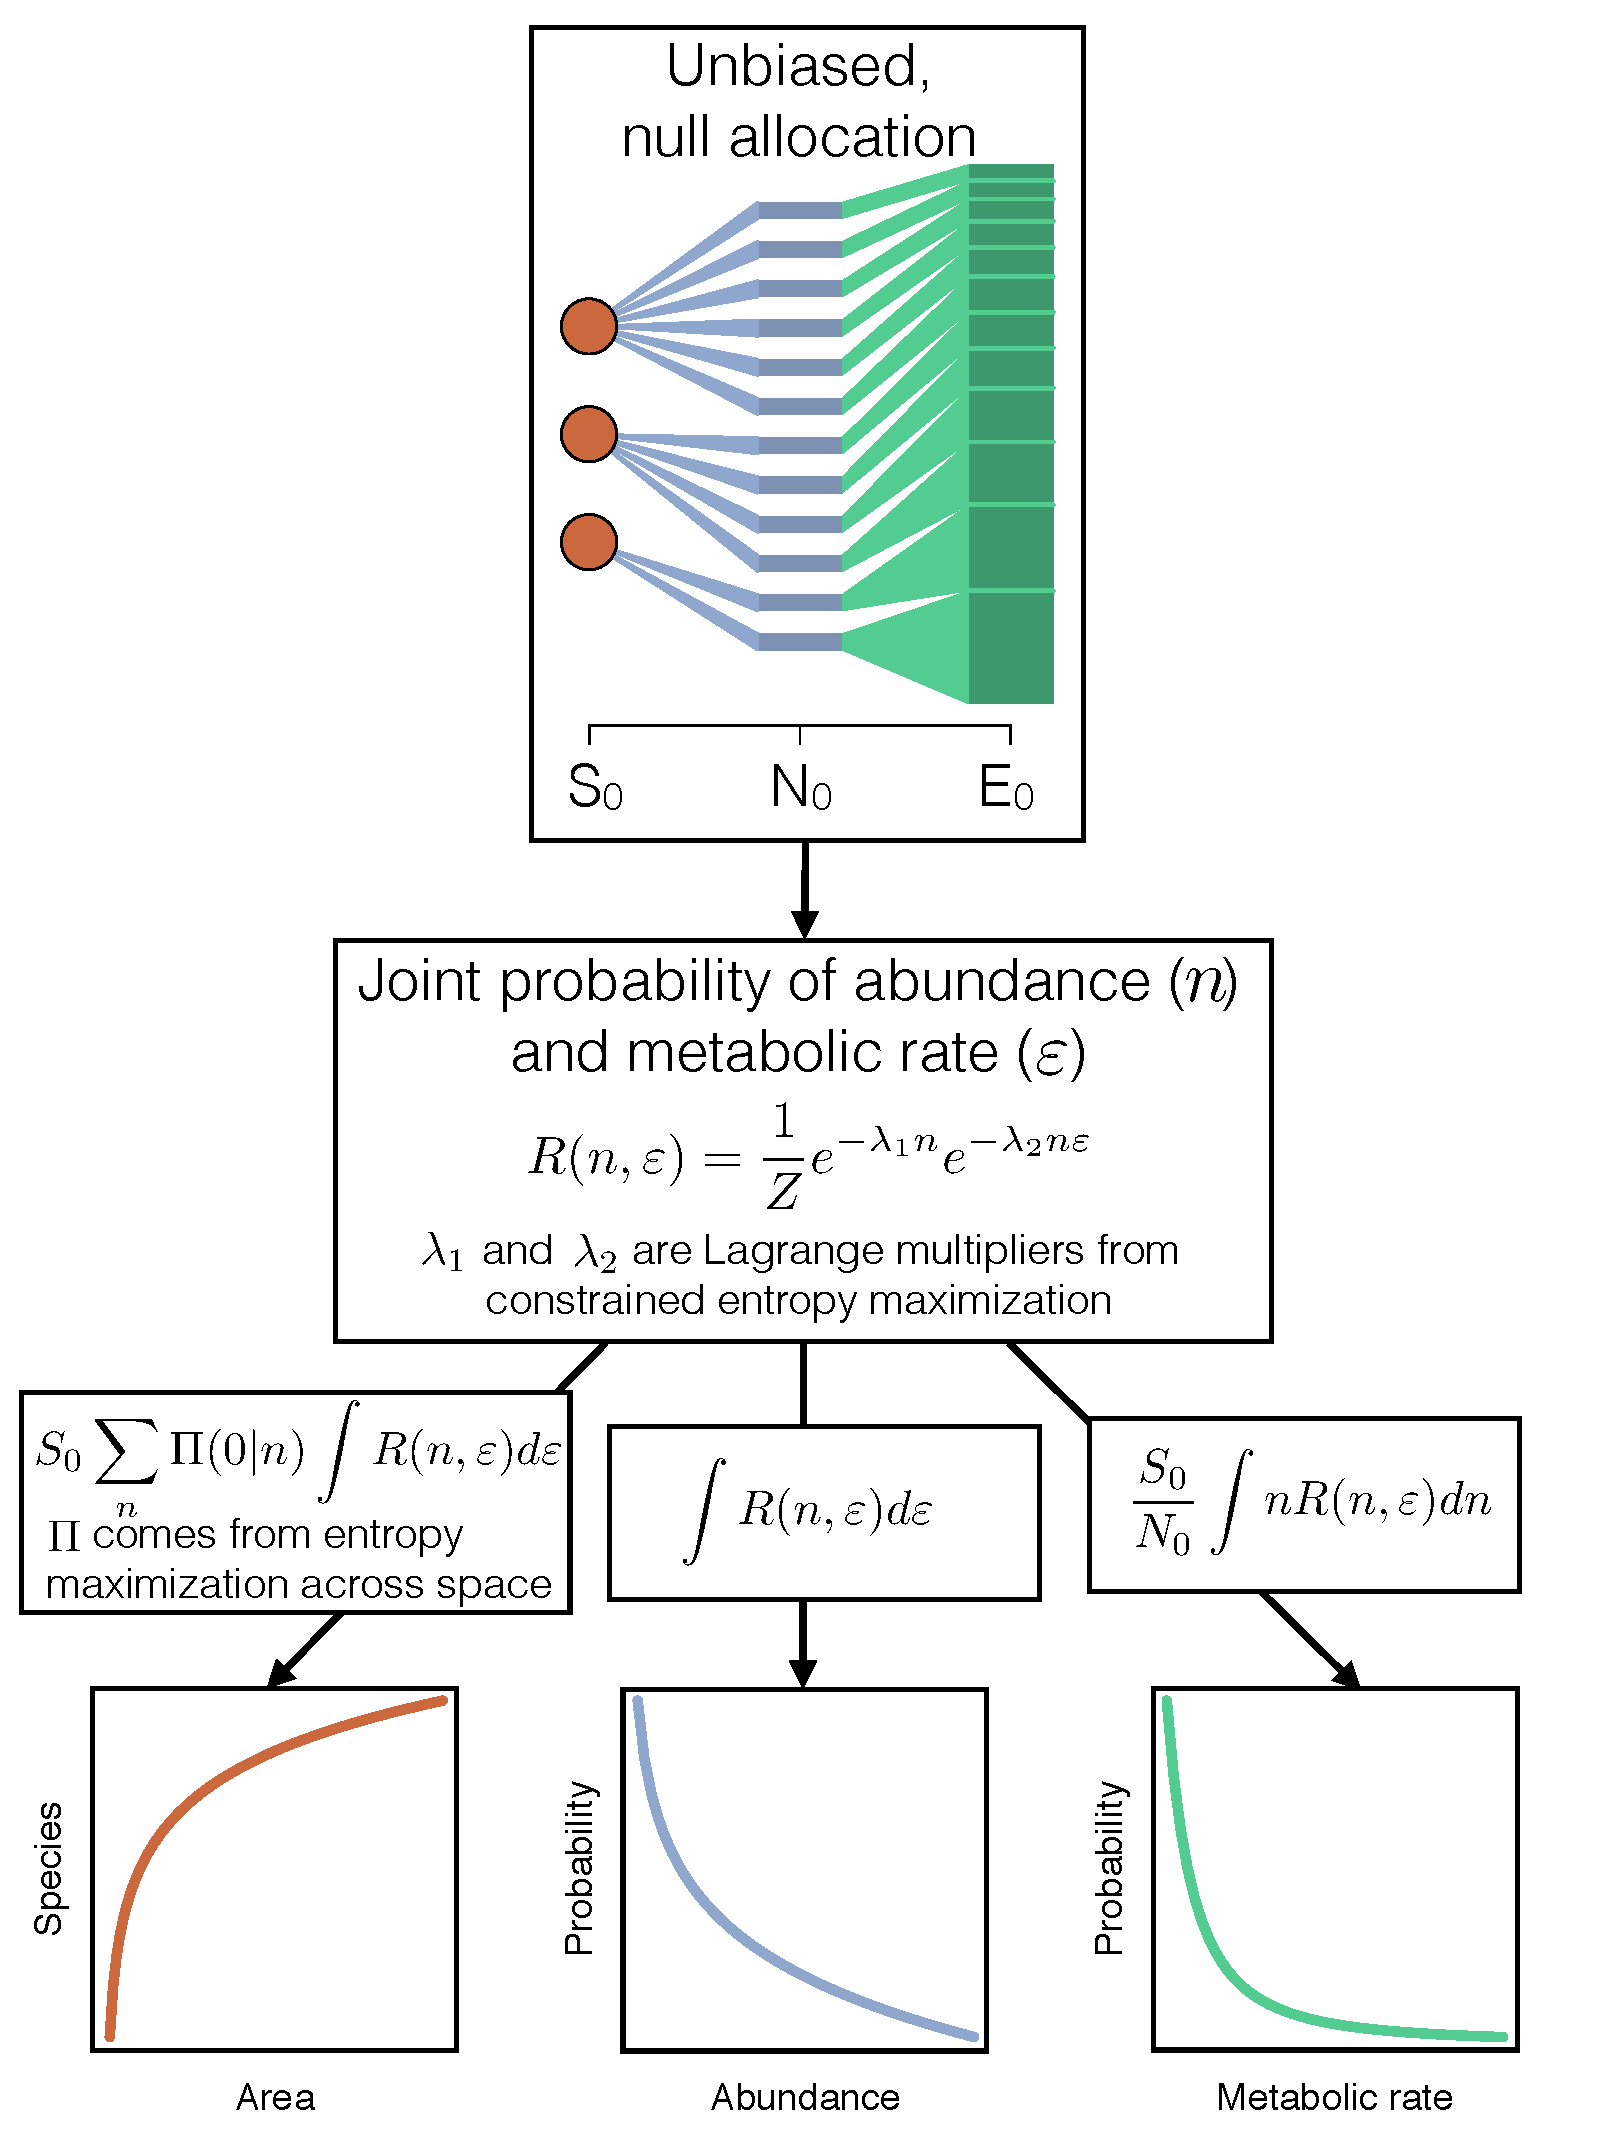
\includegraphics[scale=0.325]{../figs/fig_meteFramework.pdf}
    \end{center}
    \vspace{2pt}
  \end{minipage}
}
\vspace{-5pt}
\end{wrapfigure}

\textbf{We propose to use islands of the Hawaiian archipelago to
  understand how and why ecosystems depart from steady state and the
  consequences of these departures on biodiversity dynamics and
  invasibility.}  Remote island archipelagos provide an opportunity to
integrate ecological and evolutionary processes, advancing our
understanding of the regulation of biodiversity through the lens of
theory.  This is particularly true when the component islands are
arranged chronologically, as is found in ``hotspot'' islands that form
a geological age gradient representing snapshots of community assembly
through evolutionary time. Such islands provide simple and discrete
systems,of known age and varying area, allowing them to serve as
excellent ``natural laboratories'' for ecological and evolutionary
study in a regional context \citep{simon1987, chadwick1999,
  gillespieClague2009}. Our team has a strong foundation of research
expertise and experience across the islands on microbes (Brodie,
Ceja-Navarro), arthropods (Rominger, Gillespie, Gruner and
Krehenwinkel), plants (Chase), ecosystems (Giardina), molecular
biology (Brodie, Ceja-Navarro, Krehenwinkel), and theory (Rominger,
Chase).

%
\begin{wrapfigure}{r}{0.45\textwidth}
\vspace{-50pt}
\colorbox{gray!20}{
  \begin{minipage}{0.45\textwidth}
    \noindent    
    {\bf Box 2: Statistical Steady State} 

    A statistical steady state exists in an ecological community if
    changes in biodiversity occur slowly and in sync with
    environmental changes \citep{harte2011}. This condition is
    independent of the specific biological mechanisms mediating the
    interaction of biodiversity with its environment, so long as those
    mechanisms do not constitute information beyond the state
    variables (see Box 1) of the system. An example of such additional
    information would be specialized co-evolution between herbivores
    and plants that lead to more uniform allocation of primary
    productivity across consumers than expected by chance.  The idea
    of statistical steady state connects with previously explored
    ecological theory on stationarity and ergodicity
    \citep{maurer1999}, but is not tied to notions of equilibrium as a
    hypothesized state that ecosystem rate processes may attain or be
    driven away from \citep[e.g. not:][]{levin1970, scholz1997,
      rabosky2009}.

    The existence (or non-existence) of such steady states has wide
    ranging implications. For example, whether conservation should
    focus on conventional preservationist paradigms or adaptive
    management \citep{levin1999} depends on whether biodiversity is
    largely in statistical steady state or not. Whether biodiversity
    rapidly and consistently tends towards a steady state determines
    how species and the communities they form will respond to global
    environmental change \citep{barnosky2012}.
  \end{minipage}
}
\vspace{-10pt}
\end{wrapfigure}
%

We will characterize the ecological communities, including their
abundance, diversity, and network structure, associated with three
critical stages in nutrient cycling: 1) Living plants, the arthropods
they support and the microbes supported by both; 2) Plant and animal
detritus and its associated arthropod and microbial communities; and
3) Soil communities of arthropods and microbes.  In each of these
ecosystem domains we will use the maximum entropy theory of ecology to
characterize departure from statistical steady state.  In order to
understand the mechanistic causes of these departures we will also
evaluate how deviations from METE can be predicted by the ecology and
evolution of the organisms comprising each community, testing the
hypotheses outlined below.  We will enable this line of research by
sampling plants, arthropods and microbes across multiple spatial
scales, and across gradients of environment (precipitation and
elevation as a surrogate for temperature) and substrate age (as a
surrogate for both biogeochemical change and evolutionary
development).  We will also make use of long term fertilization
experiments \citep[see letter of
collaboration;][]{vitousek1997nutrient} to evaluate the roles of
evolutionary history versus biogeochemical processes in driving
biodiversity patterns.  Using plants, arthropods and microbes as
discrete test cases, representing a breadth of life history strategies
across the tree of life, we will test hypotheses (outlined in section
\ref{sec:hyp}) about deviations from statistical steady state based on
how organisms persist, adapt and speciate in their environments.  
{\bf In order to understand how communities are likely to change in
  response to non-analog, anthropogenically-driven climate regimes and
  across spatial scales we will build spatially explicit models that
  link the mechanistic drivers (e.g. rapid community or population
  change, and evolutionary novelty) of deviation from statistical
  steady state to remotely sensed data and detailed ecosystem
  characterizations taken at the NEON site in Hawaii, and our
  complementary sampling locations. Our project will contribute
  theoretical constructs for use across NEON sites and bioinformatic
  tools to advance the rate and dimensionality of biodiversity data
  gathered at these sites.}

\section{Proposed Research}

\subsection{Research objectives and hypotheses}

Our proposed research approach is organized in Figure
\ref{fig:research}.  We have four core research objectives:
\begin{itemize}
\item[{\bf RO1}] Describe how deviations from statistical steady state
  (measured by METE) relate to ecosystem age, environmental
  variables and invasion.
\item[{\bf RO2}] Model niches and interaction networks with respect to
  age, environment and phylogenetic information.
\item[{\bf RO3}] Combine {\bf RO1} and {\bf RO2} to model invasion
  potential and deviations from statistical steady state across
  spatial scales and into future climate scenarios.
\item[{\bf RO4}] Develop open source lab protocols and software to rapidly
  advance generation and analysis of multidimensional biodiversity
  data (taxonomic, genetic and phylogenetic) that can be applied
  across NEON sites.
\end{itemize}

We will use maximum entropy theory to identify deviation from
statistical steady state across environmental and evolutionary
gradients, and long-term experiments.  We will place these deviations
in the context of ecological and evolutionary information to
understand the mechanistic causes for deviations from statistical
steady state and its implications for invasion potential.  We will
produce detailed networks of interactions between arthropods and
plants, arthropods and microbes, and microbes and microbes to
understand how species interactions evolve and shape conformation to
or deviation from statistical steady state.  We will also reconstruct
the abiotic niches of all taxa (plants, arthropods and microbes) for
which sufficient data are available.  We will use these reconstructed
niches to understand patterns of specialization and generalization,
how these ecological states evolve, and their consequences for the
steady state of biological assemblages.  Finally, we will develop a
new bioinformatic approaches to generate massive genetic and
phylogenetic data for all communities sampled; these data will allow
us to analyze networks, niches and deviations from statistical steady
state in a phylogenetic framework to evaluate evolutionary signals in
observed patterns.

\begin{figure}[!htb]
  \centering
  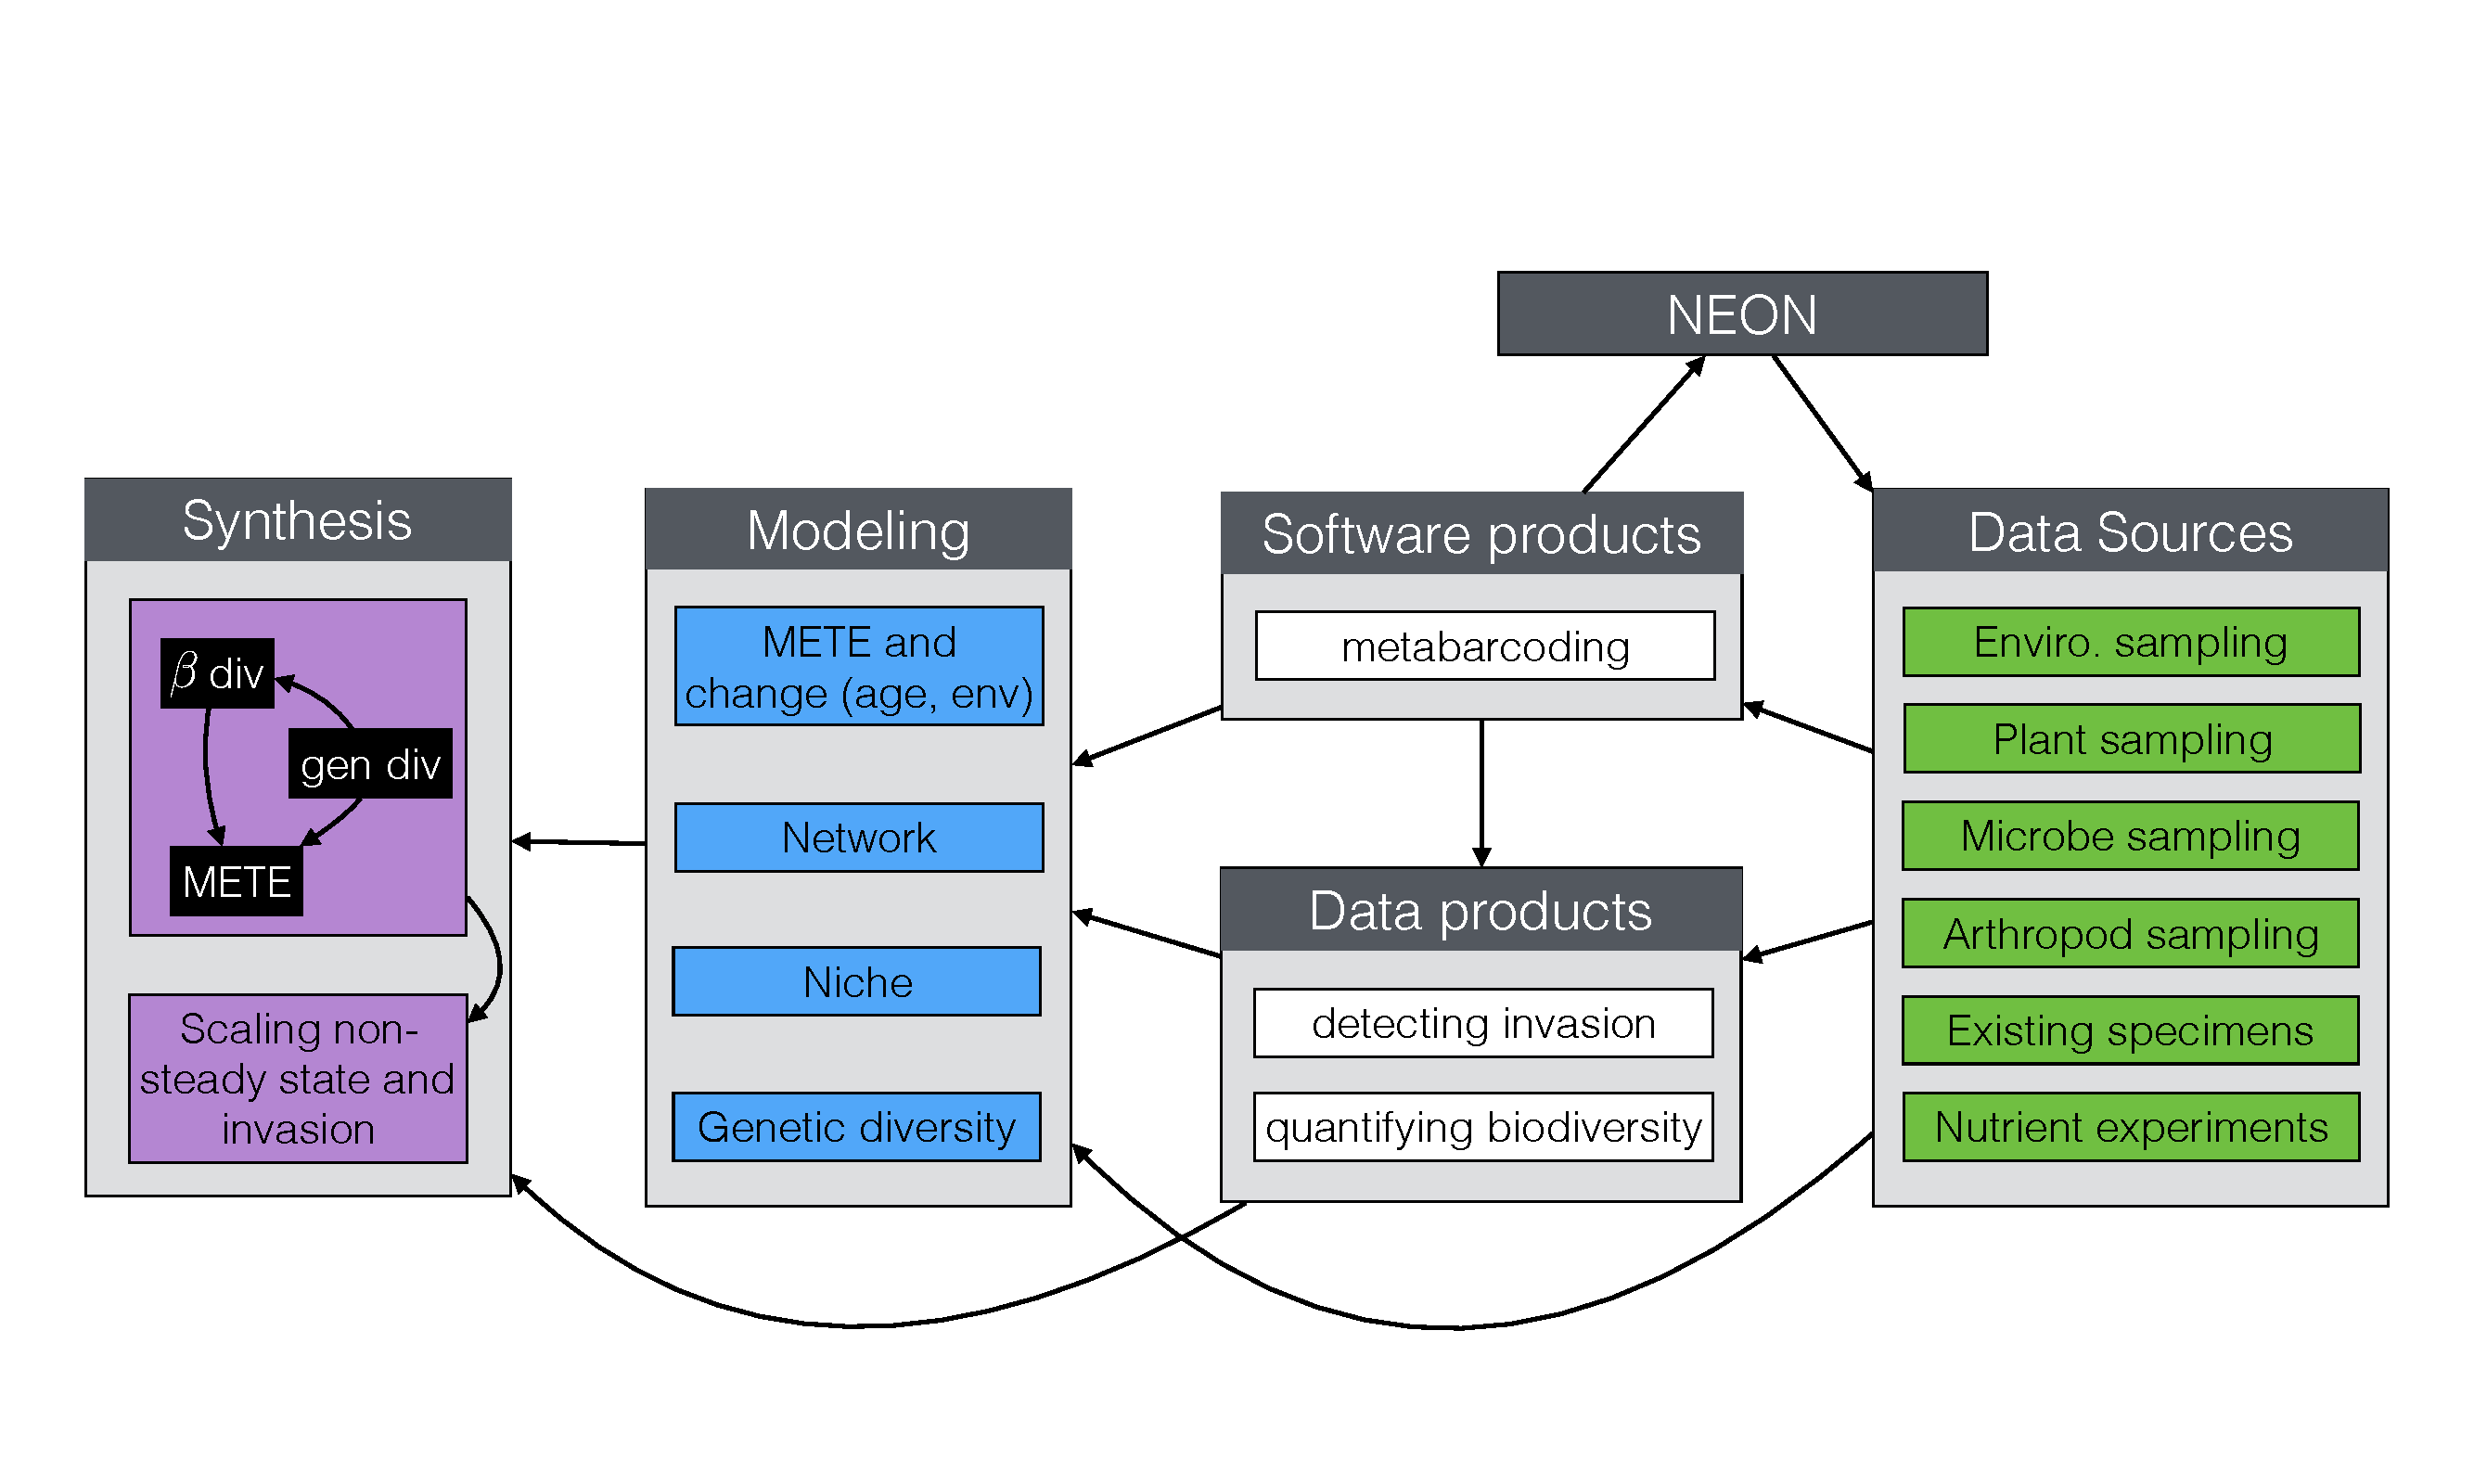
\includegraphics[scale=0.4]{../figs/fig_research.pdf}
  \caption{Conceptual network illustrating how we will achieve
    modeling and synthesis goals using diverse data resources, novel
    data and software products, and integration with the NEON site in
    Hawai'i. Synthesis approaches are further detailed in Figure
    \ref{fig:concept}.}
  \label{fig:research}
\end{figure}

To forecast these mechanistic drivers of departure from statistical
steady state into future, non-analog environments we will model
networks, niches and community phylogenetics using remotely sensed
environmental variables and detailed field measurements from the NEON
site and our complementary sampling sites.  These models will be
spatially explicit and use the framework of Bayesian hierarchical
modeling to incorporate diverse data types, including existing
biocollections data from previous NSF funded projects in Hawaii (our
Hawaii Dimensions in Biodiversity project) and specimen data curated
in State and museum databases.  To permit theory testing and modeling
across large scales we will develop a novel sequencing and
bioinformatics approach to generate massive, multidimensional
(i.e. taxonomic and genetic) biodiversity data.  We will use this
combined approach of novel theory testing and novel data generation to
test hypotheses outlined below relating departures from statistical
steady state to feedbacks between ecological and evolutionary
processes.

\subsubsection{Hypotheses}
\label{sec:hyp}

\begin{itemize}
\item Departures from statistical steady state ({\bf RO1}):
  \begin{itemize}
  \item[{\bf H1}] We predict that deviations from METE will be largely predicted by age along
    the chronosequence. These deviations will be driven primarily by
    two processes related to the evolutionary assembly of biotas: ({\bf H1a})
    primary succession (both by long distance dispersal and
    speciation) in newly formed habitats; and ({\bf H1b}) adaptive evolution
    leading to unique constraints on assembly not consistent with
    statistical steady state
    \begin{itemize}
    \item[{\bf H1a}] leads us to predict deviations from METE on young
      substrates and for generalist taxa, especially those that are
      dispersal limited (e.g. detritivores in Fig. \ref{fig:meteAll}).
      Additionally, we predict a negative correlation between the
      breadth of reconstructed abiotic niches and deviation from METE
    \item[{\bf H1b}] leads us to predict deviations in communities
      dominated by specialist taxa in old communities once they have
      established intricate evolutionary relationships with their
      coexisting species and environments (e.g. as seen in herbivores
      in Fig. \ref{fig:meteAll} and our previous published work
      \citep{rominger2015}). Based on this hypothesis we further
      predict
      \begin{itemize}
      \item a positive correlation between network specialization and
        deviation from METE
      \item a negative correlation between phylogenetic diversity and
        deviation from METE
      \end{itemize}
    \item[{\bf H1c}] Because adaptive evolution resulting in niche
      specialization and dispersal limitation both likely result in
      strong spatial structuring of communities, measures of spatial
      turnover and deviations from METE should be positively
      correlated (e.g. as seen in Fig. \ref{fig:meteExplc}).
    \item[{\bf H1d}] Because rapid population expansion, population
      contraction, limited dispersal and local adaptation all lead to
      low allelic diversity within populations
      \citep{gillespie2010popgen}, genetic diversity should be
      negatively correlated with deviation from METE.
    \end{itemize}
  \item[{\bf H2}] Given the climatic stability of Hawai'i since the
    last glacial maximum \citep{gavenda1992}, we predict deviations
    from METE should not depend on environmental variables after
    accounting for ecosystem age.  This includes the prediction that
    in long term fertilization experiments, fertilized communities
    will conform to the same patterns as their unfertilized control
    communities of the same age regardless of underlying nutrient
    availability.
  \item[{\bf H3}] However, with rapidly changing climates we do expect
    environmental variables to predict modeled deviations from
    statistical steady state. Specifically, with the creation of novel
    environments and loss of existing environments due to
    anthropogenic climate change, we expect rapid population changes
    and exacerbated constraints on movement due to unique evolutionary
    adaptations to previously stable environments.  Thus we predict
    novel climatic conditions to drive future deviations from
    METE. Modeling this prediction corresponds to {\bf RO3}.
  \item[{\bf H4}] We predict that in disturbed systems, statistical steady
    state will be achieved only through rapid assembly of novel
    ecosystems (i.e. communities dominated by highly vagile invasive
    taxa).  Thus deviations from statistical steady state are expected
    to promote invasion, while invasion itself will tend to return
    systems to statistical steady state.  This hypothesis leads to
    further hypotheses:
    \begin{itemize}
    \item[{\bf H4a}] Community phylogenetic, niche occupancy and network
      position of invasive species will be similar to generalist taxa
      that form communities conforming to METE
    \item[{\bf H4b}] Models including level of invasion as an
      explanatory variable will help explain deviations from METE that
      cannot be otherwise explained by age and environment.
    \item[{\bf H4c}] Repeated surveys of communities will show that
      systems previously deviating from statistical steady state in
      prior censuses now contain higher proportions of invasives
      compared to those closer to statistical steady state.  This
      hypothesis cannot yet be tested, but our proposed research lays
      the groundwork for long term ecological monitoring.
    \end{itemize}
  \end{itemize}
\item Evolution of niches and networks ({\bf RO2})
  \begin{itemize}
  \item[{\bf H5}] We predict that niches will become more constrained
    across evolutionary time, leading to the further predictions that:
    \begin{itemize}
    \item[{\bf H5a}] reconstructed niches will be smaller for taxa endemic to older islands
    \item[{\bf H5b}] spatial turnover will be stronger across gradients on older islands
    \item[{\bf H5c}] networks will become more specialized across
      evolutionary time \citep[supported by our previous work on
      network evolution][]{rominger2015}
    \end{itemize}
  \item[{\bf H6}] We predict that closely related taxa will overlap in
    niche space if they occupy broad distributions across abiotic
    environments and generalist network positions, whereas specialist
    taxa will show phylogenetic signals of over-dispersion owing to
    adaptive differentiation.
  \end{itemize}
\end{itemize}

Tests of the first four hypotheses ({\bf H1}--{\bf H4}; {\bf RO1})
will be used to understand how deviations from statistical steady
state result from the evolutionary and ecological characteristics of a
community.  Tests of hypotheses {\bf H5} and {\bf H6} ({\bf RO2}) will
be used to illuminate how those eco-evolutionary drivers themselves
respond to environmental constraints across space and through
evolutionary time.  Quantifying these eco-evolutionary patterns and
mechanisms is permitted by {\bf RO4}. Combining the insights of both
sets of hypotheses will allow us to model deviations from statistical
steady state and resultant changes in invasion potential across space
and into future climate scenarios ({\bf RO3}).


\begin{figure}[!htb]
  \centering
  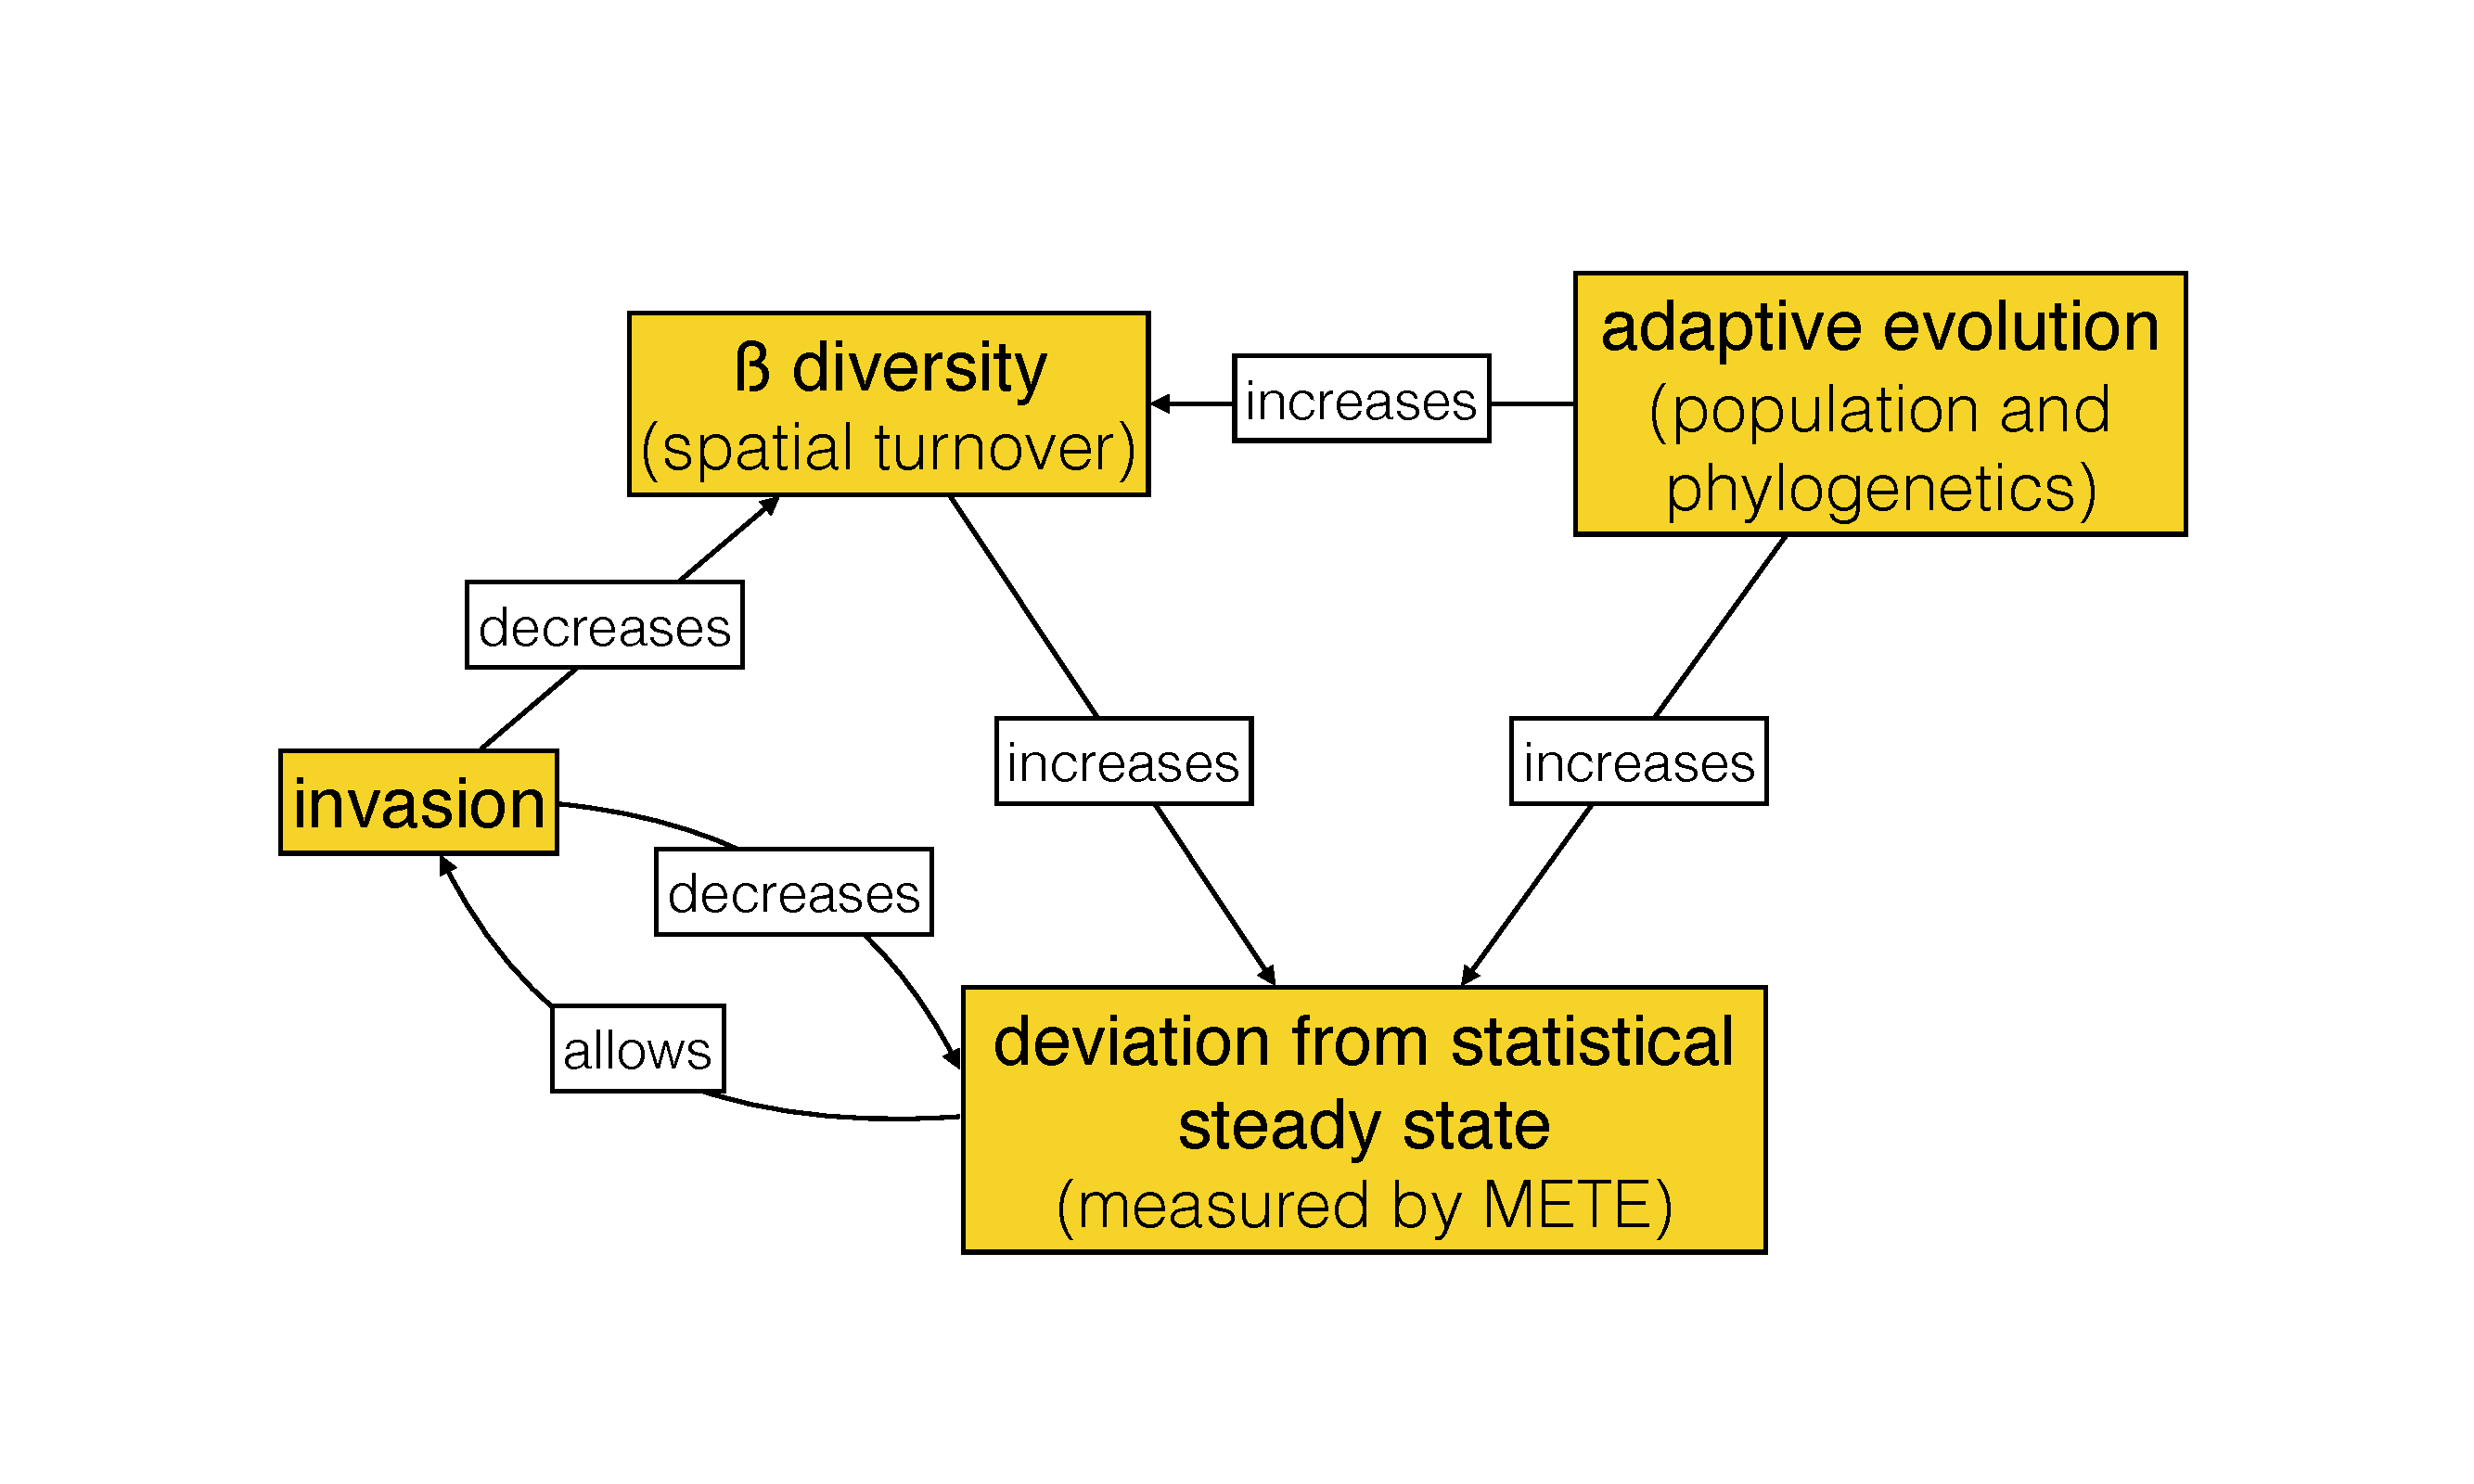
\includegraphics[scale=0.3]{../figs/fig_concept.pdf}
  \caption{Network illustrating hypotheses as connections between core
    components of the proposed research. In order to scale deviations
    from statistical steady state and invasion potential across space
    we will model the drivers of changes in spatial turnover and
    phylogenetic signal---evolution of niches and networks.}
  \label{fig:concept}
\end{figure}

\subsection{Significance and Rationale}

Understanding how environmental change will alter the feedback between
ecology and evolution and drive biodiversity out of statistical steady
state is at the core of our proposal.  Using METE to capture
statistical steady state and understand deviations from it promises to
be a powerful diagnostic tool in evaluating ecosystems nearing tipping
points.  Hawaii is an ideal study system to realize this potential due
to its varying chronology (allowing tests of theory in communities of
different stages of evolutionary development) and due to its
replicated environmental gradients across this chronology (see
Fig. \ref{fig:map}. The NEON site at Pu'u Maka'ala Natural Area Reserve
on Hawai'i Island will provide the core measures needed to quantify
the abiotic environment.  We will replicate these measurements across
gradients of elevation and precipitation, using ground-truthed
remotely sensed measurements to provide both fine grain and
broad-scale environmental data products.  These combined sampling
sites lay the groundwork for significant long-term ecological
monitoring.

The same ability to generate massive amount of environmental data via
remote sensing does not exist for organismal ecology and evolution.
As part of our Dimensions in Biodiversity grant, Rominger and
Krehenwinkel are developing laboratory and bioinformatic methods to
obtain sequence data, and estimates of abundance and biomass for
thousands to millions of arthropods collected via ecological sampling.
As part of the current proposal this promising new approach will be
developed into an open source lab protocol and software package that
can be distributed across all NEON sites.

\begin{figure}[!htb]
  \centering
  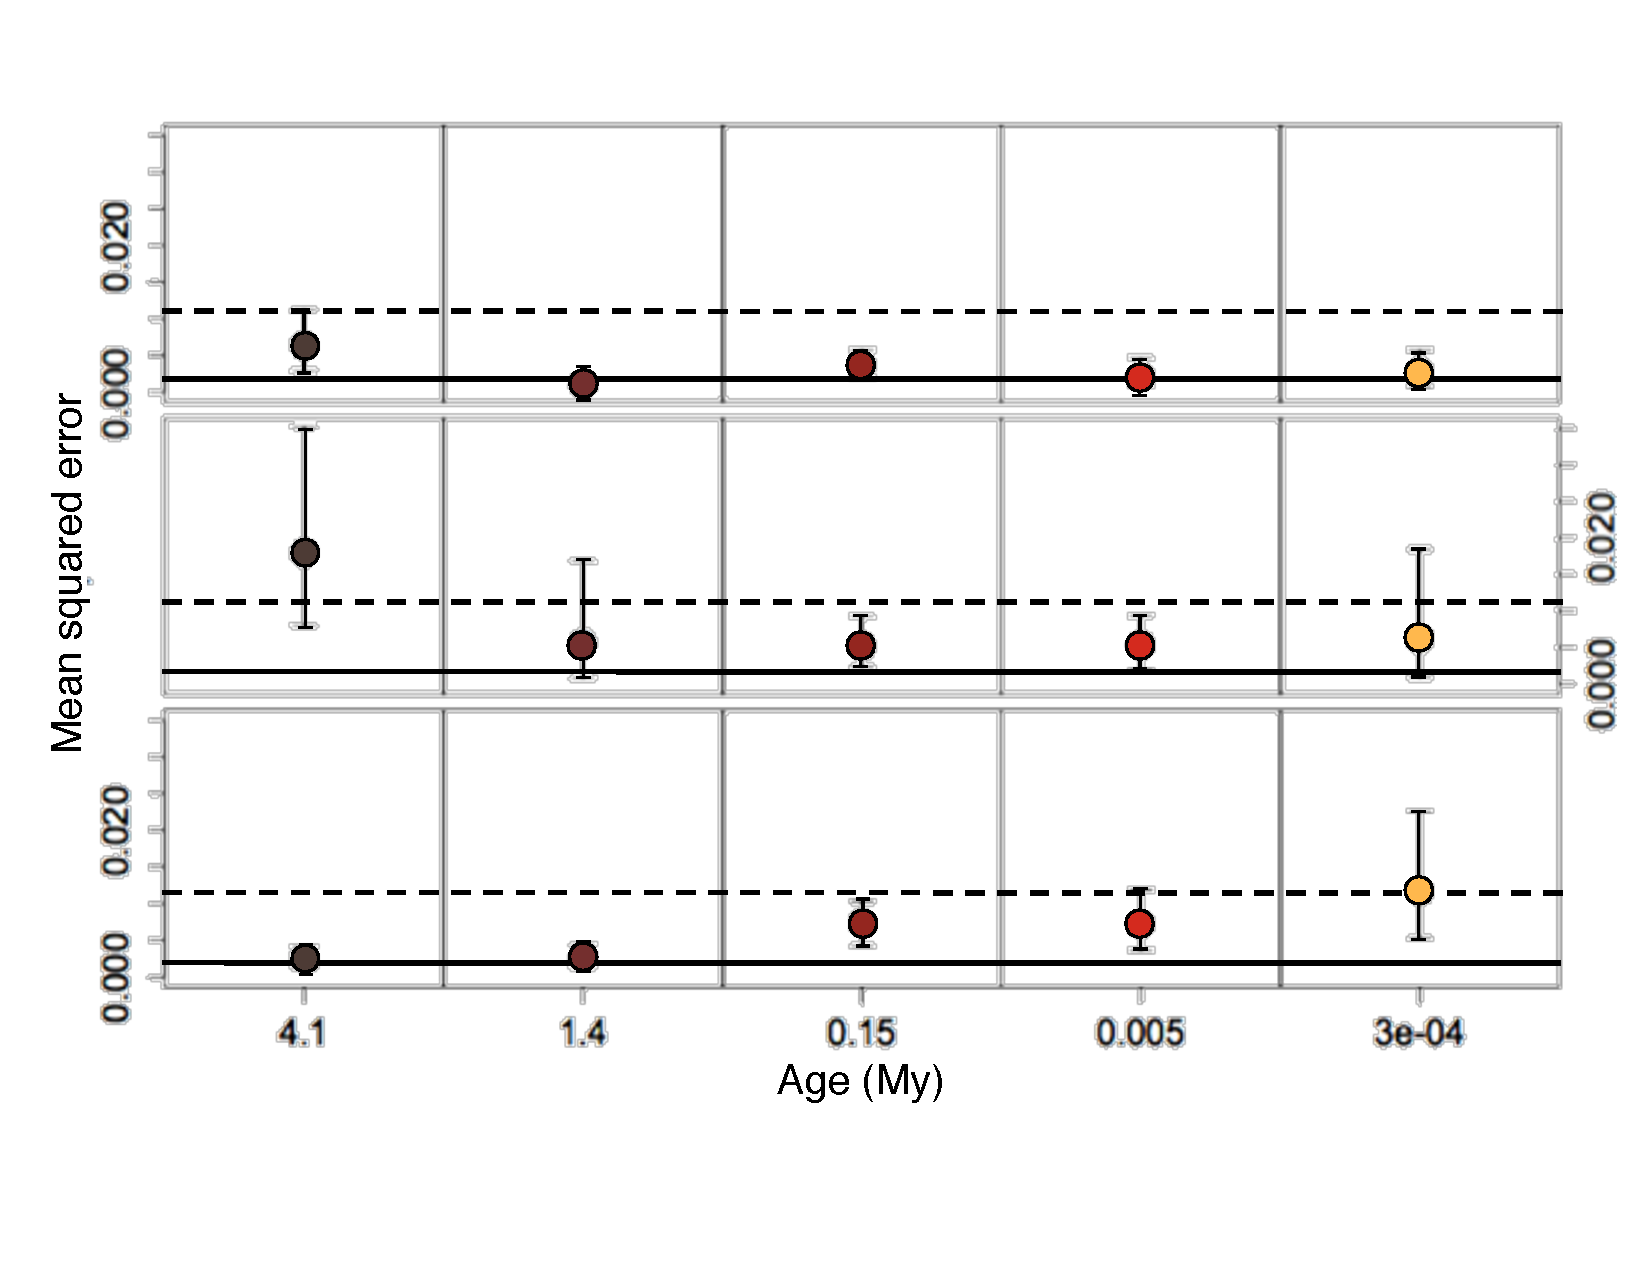
\includegraphics[scale=0.4]{../figs/fig_meteAll.pdf}
  \caption{Deviations from METE (measured as mean squared error)
    across the Hawaiian chronosequence (colors correspond to ages in
    Fig. \ref{fig:map}) for three different arthropod guilds
    \citep[data from][]{gruner2007}.  Dashed line represents
    statistical grounds for rejecting METE. Note that predatory
    arthropods have high dispersal ability and low population genetic
    structure compared to detritivorous arthropods
    \citep{rominger2015}, which explains greater deviations from
    statistical steady state in detritivores, especially in younger
    aged ecosystems.  The poor fit of herbivores in older ecosystems
    is likely due to their unique evolution with host plants,
    corroborated in our study of network structure across the
    chronosequence \citep{rominger2015}.}
  \label{fig:meteAll}
\end{figure}

Our use of METE as a diagnostic tool has been corroborated in the
Hawaiian system with previous and current work.  Rominger, with
Gillespie, Gruner, and Harte as collaborators and co-authors, has
shown that deviations from METE show consistent patterns across the
chronosequence for different arthropod guilds with different life
history characteristics (Fig. \ref{fig:meteAll}).  Additionally, these
patterns can be predicted by the amount of spatial turnover in species
composition between sites, and by the proportion of the community
dominated by invasive species (Fig. \ref{fig:meteExplc}). This work
confirms our hypotheses that deviations from statistical steady state
can be predicted by limited dispersal and niche partitioning (leading
to increased spatial turnover) and that deviation from statistical
steady state is related to invisibility of ecosystems.  Our proposed
work will extend this approach by explicitly testing more nuanced
hypotheses about the role of evolutionary processes in driving these
non-steady state observations and extending these predictions across
space and into future environments with hierarchal models.

\begin{figure}[!htb]
  \centering
  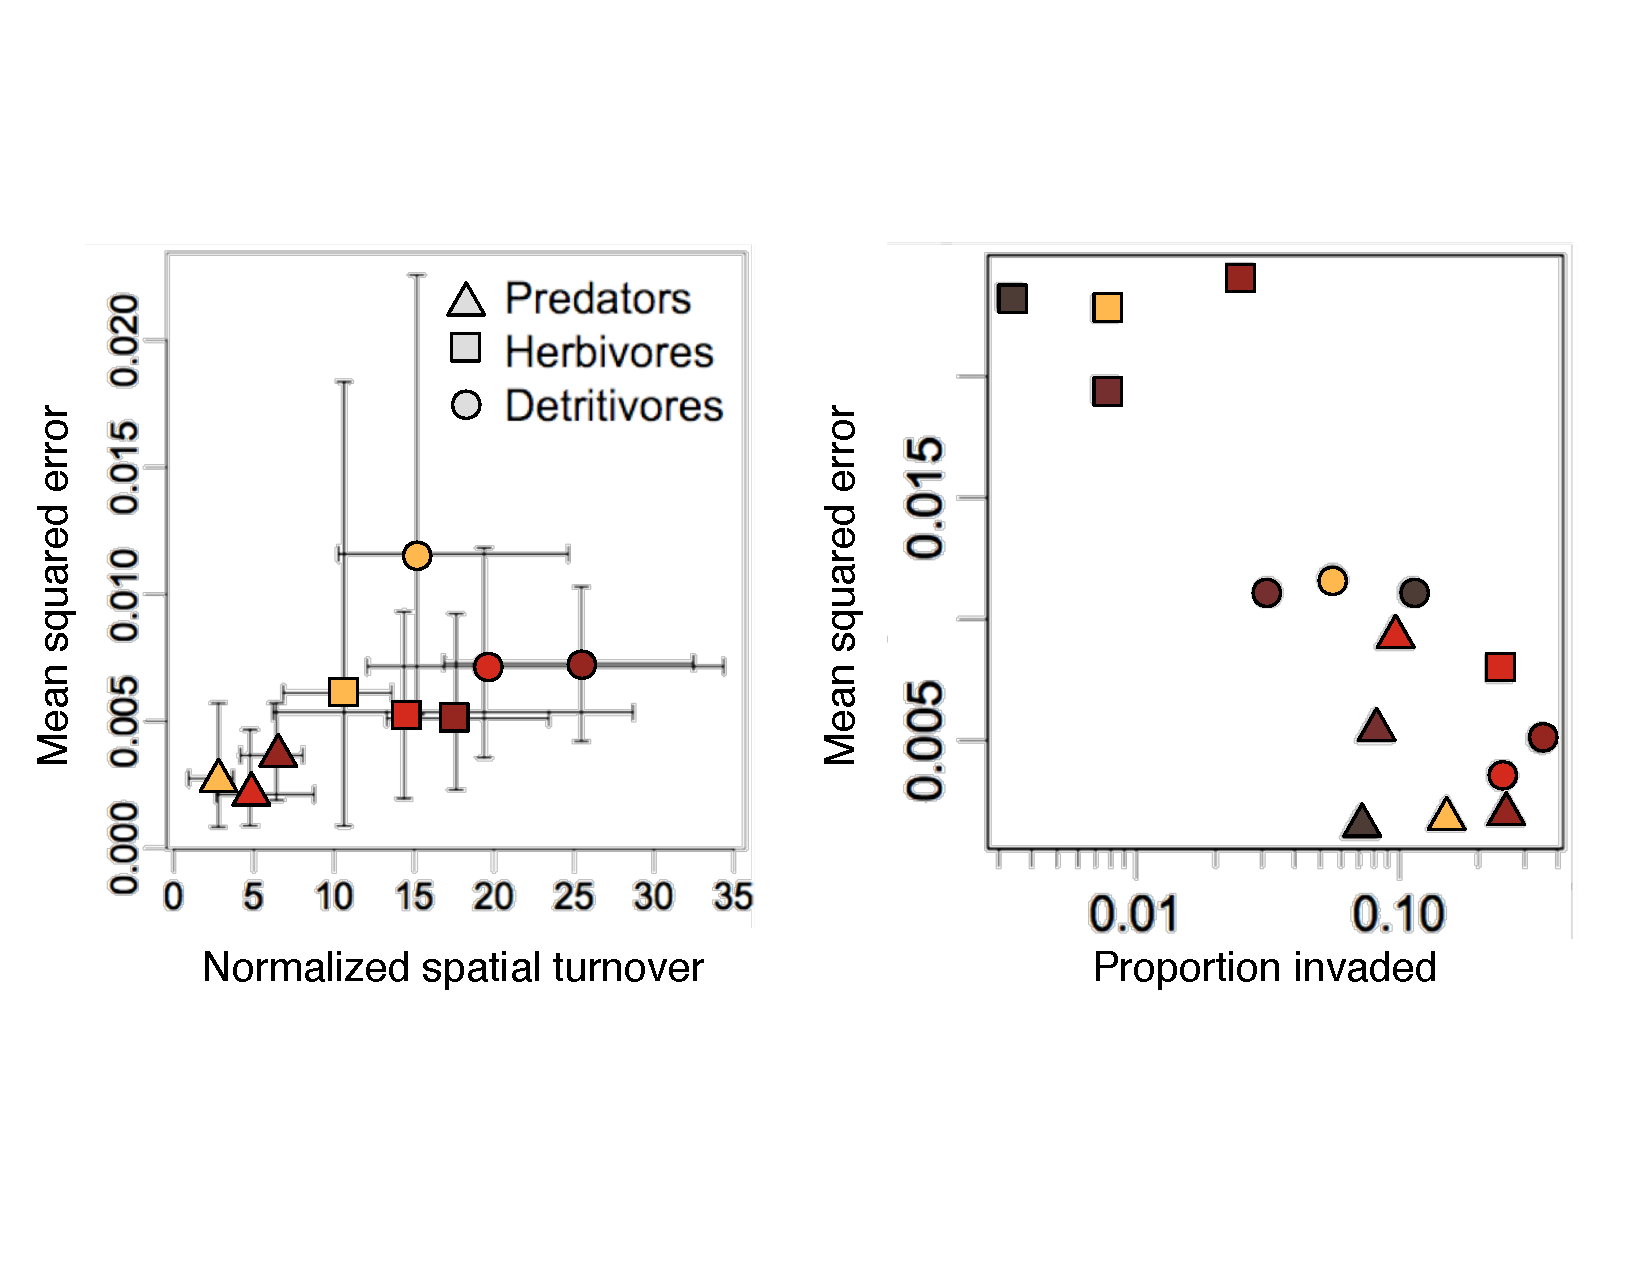
\includegraphics[scale=0.4]{../figs/fig_meteExplc.pdf}
  \caption{Across arthropod guilds and substrate ages (colors
    correspond to age in Fig. \ref{fig:map}) deviations from METE
    (measured as mean squared error of METE predictions) are predicted
    by spatial turnover is species composition (left panel).  More
    heavily invaded systems conform best to METE (right panel)
    suggesting that invasion acts to bring non steady state systems
    back into steady state by an influx of highly vagile, generalist
    invasive species. Data from \citep{gruner2007}.}
  \label{fig:meteExplc}
\end{figure}

\subsection{Methods}

\subsubsection{Integration with NEON and sampling design across
  environmental and age gradients}

\paragraph{NEON site.}
The goal of NEON is to provide ecological data at multiple spatial and
temporal scales. Our plan is anchored with the Pu'u Maka'ala Natural
Area Reserve on the Mauna Loa volcano on the Big Island of Hawaii
(19.553\textdegree, -155.317\textdegree; Fig. \ref{fig:map}), a Core
Terrestrial site with the launch date planned for 2017. The site
represents montane wet forest with mostly native vegetation dominated
by the endemic tree, {\it Metrosideros polymorpha}
(Myrtaceae). However, 95\% of the world's terrestrial climates
are represented in the greater region of the Hawaiian archipelago
\citep{juvik1998}, and a single site will fail to characterize this
tremendous diversity in climate, habitats and species composition. By
replicating core NEON protocols at carefully selected sites with
orthogonal variation in temperature and precipitation, along a
geological chronosequence representing evolutionary time, the Hawaiian
macrosystem will yield the precision of NEON measurements to test
ecological theory and to predict consequences of future changes in
climate. We aim to combine data to be collected by NEON with data from sites
across the Hawaiian Islands, in order to understand regional-scale
ecological processes and how these respond to change over space and
time.


\paragraph{Complementary sites.}
We will collect data in an explicit, nested design that allows
integration with the NEON-generated data, while using data from the
entire terrestrial region of the Hawaiian Islands to provide
information on processes of several groups of organisms across
multiple scales. Data will be gathered across elevation and
precipitation gradients from evolutionarily old, middle aged and young
islands (Kaua'i: 4--5 my; Maui: 1--1.5 my; and Hawai'i: 0.001--0.5
my).  On each island we will establish 6 sites (1 ha in size): 3 along
a windward (i.e. high precipitation) elevation gradient and 3 along a
leeward (i.e. low precipitation) elevation gradient
(Fig. \ref{fig:map}).  Windward sites will be constrained to be within
4000--5000 mm annual precipitation, while leeward sites will be
constrained to be within 1500--2500 mm annual precipitation.  We will
consider an elevation gradient from 900 -- 2500 m elevation.  On
Hawai'i Island we will use the area adjacent to the Pu'u Maka'ala NEON
site as one of these 6 sites.  Each site will consist of 3 replicate
plots to insure thorough coverage of local variation. The sampling
locations and design are given in Figure \ref{fig:map}.


\begin{figure}[!htb]
  \centering
  \includegraphics[scale=0.45]{../figs/fig_bigMap.pdf}
  \caption{Map of Hawai'i showing chronological age, elevation, and
    precipitation.  Gray dots represent sampling locations with
    existing data from our Dimensions in Biodiversity project.
    Triangle corresponds to the NEON site at Pu'u Maka'ala.  Regions
    delineated with rectangles represent proposed areas where sampling
    sites will be established (6 per island). Black squares in the
    detail map represent potential sampling sites complementing the
    NEON site.  In the detail map, precipitation is color coded as
    before, but elevation is shown as 200 m contours. Sites will be
    organized in a nested fashion.  Green plots represent our
    stratified sampling plots within a site, brown quadrats correspond
    to litter and soil sampling quadrats, and the blue 10 cm x 10 cm
    sub quadrant corresponds to our microbial samples.  Orange dots
    represent locations of temperature and humidity data loggers, in
    addition to litterfall collection locations.}
  \label{fig:map}
\end{figure}


\paragraph{Sampling approach and collection of organismal data.}
We will select sites in clearly defined ohia/koa montane, wet and
mesic forest communities. The rationale here is that (i) Ohia
({\it Metrosideros polymorpha}) is the dominant canopy tree in these
forests, forming a nearly continuous layer, with patches of
sub-dominant koa ({\it Acacia koa}) and numerous associated understory
trees, shrubs, herbs, and ferns. This forest type (and the presence of
{\it Metrosideros} in particular) has been used as an important landscape
feature in our ongoing work through the Hawaii Dimensions of
Biodiversity, as it has for a generation of studies on long-term
ecosystem development. This constrains sampling to vegetation and
soils of similar physiognomy and evolutionary history, while allowing
major climatic state factors to vary. (ii) The proposed NEON site is
characterized by this forest type. Finally, (iii) {\it Metrosideros} growth
rate, growth form and chemical composition (all detectable by various
satellite and airborne spectroscopic techniques \citep{asner2006,
  asner2009, asner2012} reflects the coupled but nonlinear effects of
ecosystem age and fertility, which in turn affects the community of
organisms in a given forest stand \citep{crews1995,
  gruner2007}. Differences in plant traits can affect the structure of
an entire food web through a series of direct and indirect effects
\citep{gruner2005, bukovinszky2008}.

Figure \ref{fig:map} details the proposed layout of our sampling
plots. Within each 1-ha site, we will establish three 20 m by 20 m
plots to be selected as representative of forest height mean, maximum,
heterogeneity found in that 1-ha site. Each plot will be further
gridded into 4 m quadrats (100 in total).  Within each quadrant we
will record all tree species $\geq 1$ cm at breast height.  Within
three randomly selected quadrats we will also sample all herbaceous
species.  We will sample all arthropods within each quadrant using
timed beating (24 seconds per quadrant).  Within the same three
randomly selected quadrats used for herbaceous plant surveys we will
also extract arthropods using Berlese funnels from litter and soil
samples, gridded to 1 m$^2$ cells (in keeping with the ground beetles
collected at the NEON site).  Arthropods will be collected into
RNAlater to preserve their DNA and RNA as well as the DNA and RNA of
their associated microbes and gut contents.  While NEON protocols
focus on ground beetles (Carabidae), mosquitoes (Diptera: Culicidae),
and ticks (order Ixodida), our study will include all arthropods
because ground beetles constitute an eclectic group of lineages, most
often arboreal and unevenly distributed across the main islands
\citep{Liebherr2000}, and there are no native mosquitoes or ticks
\citep{nishida2002}.

Microbial richness and abundance will also be sampled in a gridded
design (Fig. \ref{fig:map}).  Within the three randomly selected
quadrats used for herbaceous plants, litter and soil sampling, we will
take a soil sample 100 cm in surface area (10 cm by 10 cm) and 10 cm
deep.  In the lab this will be divided into a regular 2 cm grid and
each will be sequenced.  

In all systems, microbial diversity will focus primarily on the Domain
Bacteria due to its phylogenetic breadth, and metabolic and
respiratory plasticity. Bacterial diversity will be estimated using
molecular tools to sequence 16S rRNA gene biomarkers in multiplex
using a barcoding approach. DNA extraction and 16S rRNA gene
amplification and Illumina sequencing will be carried out according to
Earth Microbiome Project standards
(\url{www.earthmicrobiome.org/emp-standard-protocols}). Ancillary
and meta data collection standards will follow the NEON the soil
microbial data collection and metadata tracking worksheet
(\url{goo.gl/nE9zPk}).  Microbial 16S rRNA gene data will be
analyzed according to \citet{shi2015}. Richness will be estimated
using both taxonomic (OTUs) and phylogenetic (Faith's phylogenetic
distance) metrics. Absolute bacterial abundances will be determined
using quantitative PCR as described in \citep{shi2015} while relative
abundances of bacterial taxa will be determined based on the fractions
of sequence reads assigned to each taxon using adjustments for rRNA
gene copy number \citep{kembel2012}.  In order to relate bacterial
taxa to metabolic rate we will use observed relationships between rRNA
copy number, genome size and metabolic rate \citep{delong2010}.

\paragraph{Environmental and biogeochemical data.}
In order to characterize the environment experienced by our focal
organisms and model deviations from statistical steady state,
achieving research objectives {\bf RO1}--{\bf RO3}, and testing
hypotheses {\bf H1}--{\bf H6}, we will replicate select NEON
measurements and instrumentation, and make use of remotely sensed data
products.

\begin{enumerate}
\item Plot-level measurements: In each microbial sampling quadrant we
  will deploy data loggers to record air temperature and moisture
  content.  We will similarly deploy data loggers to record soil
  temperature and moisture.  We will also measure soil physical
  characteristics, pH, total carbon, nitrogen, phosphorous and sulfur.
  We will measure monthly litterfall using litter traps as a surrogate
  for nutrient cycling \citep{austin2000, giardina2004} in addition to
  litter chemistry (pH, total carbon, nitrogen, phosphorous and
  sulfur) in keeping with protocols at the core NEON sites \citep{NEON}.
\item Remote Sensing and Airborne Observation Platform: We will make
  use of both existing \citep[e.g.,][]{asner2006, asner2016} and
  planned airborne remote sensing data which can provide information
  on vegetation composition and land cover and will be used in
  particular to examine the complex mosaic of forest structure and
  composition. The NEON Airborne Observation Platform (AOP) measures
  vegetation biochemical and biophysical properties with spectroscopy,
  vegetation structure and biomass with LiDAR, and produces high
  resolution imagery that can be subject to analyses of land use and
  relative cover \citep{NEON}. The combination of detailed field
  measurements at the NEON site (several of which we will replicate)
  and broad coverage remote sensing will allow use to develop
  spatially highly resolved surrogates for biogeochemical processes
  and abiotic environmental variables across the Hawaiian islands,
  following known approaches with which Giardina is integrally
  involved \citep[e.g.,][]{broadbent2014, asner2016}.  These spatial
  products, both derived by NEON and adapted by our interdisciplinary
  group, will be used to achieve {\bf RO1} and {\bf RO2}---modeling statistical
  steady state and its eco-evolutionary drivers across space.
\end{enumerate}



\subsubsection{Modeling evolutionary and environmental drivers of
  assembly}


\paragraph{Maximum entropy theory of ecology across gradients of
  environment and age}

To test our hypotheses relating age, environment and
organism/community traits to deviations from METE ({\bf RO1} and {\bf
  H1}--{\bf H4}) we will use the {\tt R} package {\tt meteR}
\citep[developed by Rominger][]{rominger2016} to evaluate the goodness
of fit of METE for soil microbes, arthropods, plants, and microbial
associates of arthropods and plants at our sampling sites across
gradients of precipitation, elevation and age.  Goodness of fit will
be measured as the normalized log likelihood squared \citep[described
in][]{rominger2016}. Using generalized linear models we will evaluate
how the goodness of fit varies between major groups (microbes,
arthropods and plants) and as a function of the underlying age and
environment of each site.

To further explore the relative importance of age as a proxy for
evolution versus biogeochemical environment (hypothesis {\bf H2}) we will
use Vitousek's long term fertilization experiments \citep[see letter
of collaboration;][]{vitousek1997nutrient} to test whether alleviating
nutrient limitations in old and young plots changes the the way in
which arthropod and microbial communities deviate or conform to METE.


\paragraph{Modeling niches, networks and community phylogenetics
  across space and evolutionary time}

We will develop a Bayesian hierarchical modeling framework to
understand how ecological and evolutionary drivers of deviations from
statistical steady state depend on local and regional environments
({\bf RO2} and hypotheses {\bf H5}--{\bf H6}).  In all models we will
incorporate explanatory environmental variables as spatial averages
with an exponentially decaying distance weighted function.  Each
variable will receive maximum weight at the point location of the
specimen and exponentially less weight as distance from the point
location increases.  The exponential rate of decay will be fit as a
free parameter in our Bayesian hierarchical model.

We will use island age as an explanatory variable interacting with
environment to evaluate how the niche occupancy and network position
of each species changes with evolutionary age (hypothesis {\bf H5}).
Because we will have phylogenetic data from metabarcoding for all
species we will evaluate patterns of niche occupancy and network
position in a phylogenetic framework, testing hypotheses of whether
closely related taxa overlap or diverge in niche occupancy, and
whether more recently diverged species tend to be generalists or
specialists (hypothesis {\bf H6}).

To test whether the niche spaces of taxa change across the
chronosequence we will build probabilistic niche models for all
species of plants and arthropods with sufficient data ($n \geq 15$
points per island).  We will use data sources from our gradient plots,
plots from our Hawaii Dimensions in Biodiversity project, digitized
museum specimens and species occurrence data made available reporting
by the Hawaii Division of Land and Natural Resources.  Because the
nature of these data is variable (abundance and presence-only) we will
use Bayesian hierarchical models to combine them into one analysis
\citep{hsdm}.  We jointly model the niches of all species in this
hierarchical approach.

To test how networks evolve across the chronosequence we will quantify
network structure using four complementary approaches: 1) deviation
from the maximum entropy predictions; 2) classic ecological network
metrics of nestedness and modularity; 3) network dissimilarity; and 4)
network specialization.  We will again take a phylogenetic approach to
evaluate how changes in network position of taxa and changes in
overall structure of networks relates to the phylogenetic distance
between component taxa.


\subsubsection{Projecting deviations from statistical steady state
  into the future}

Once we understand the connections between network structure, niche
occupancy, population size change, evolutionary diversification and
deviation from statistical steady state, we can use our models for
niches, networks, and their phylogenetic context to project these
drivers into the future, predicting where (at a regional scale)
statistical steady stead will be violated ({\bf RO3}).  Using our
understanding of how statistical steady state contributes to
invasibility of a community ({\bf RO1} and hypothesis {\bf H4}) we
will also be able to model invasion risk across scales and into future
climate scenarios.

\subsubsection{Quantifying evolutionary and macroecological patterns
  using metabarcoding}

%
\begin{wrapfigure}{L}{0.5\textwidth}
  \label{fig:metab}
  \vspace{-10pt}
  \begin{center}
    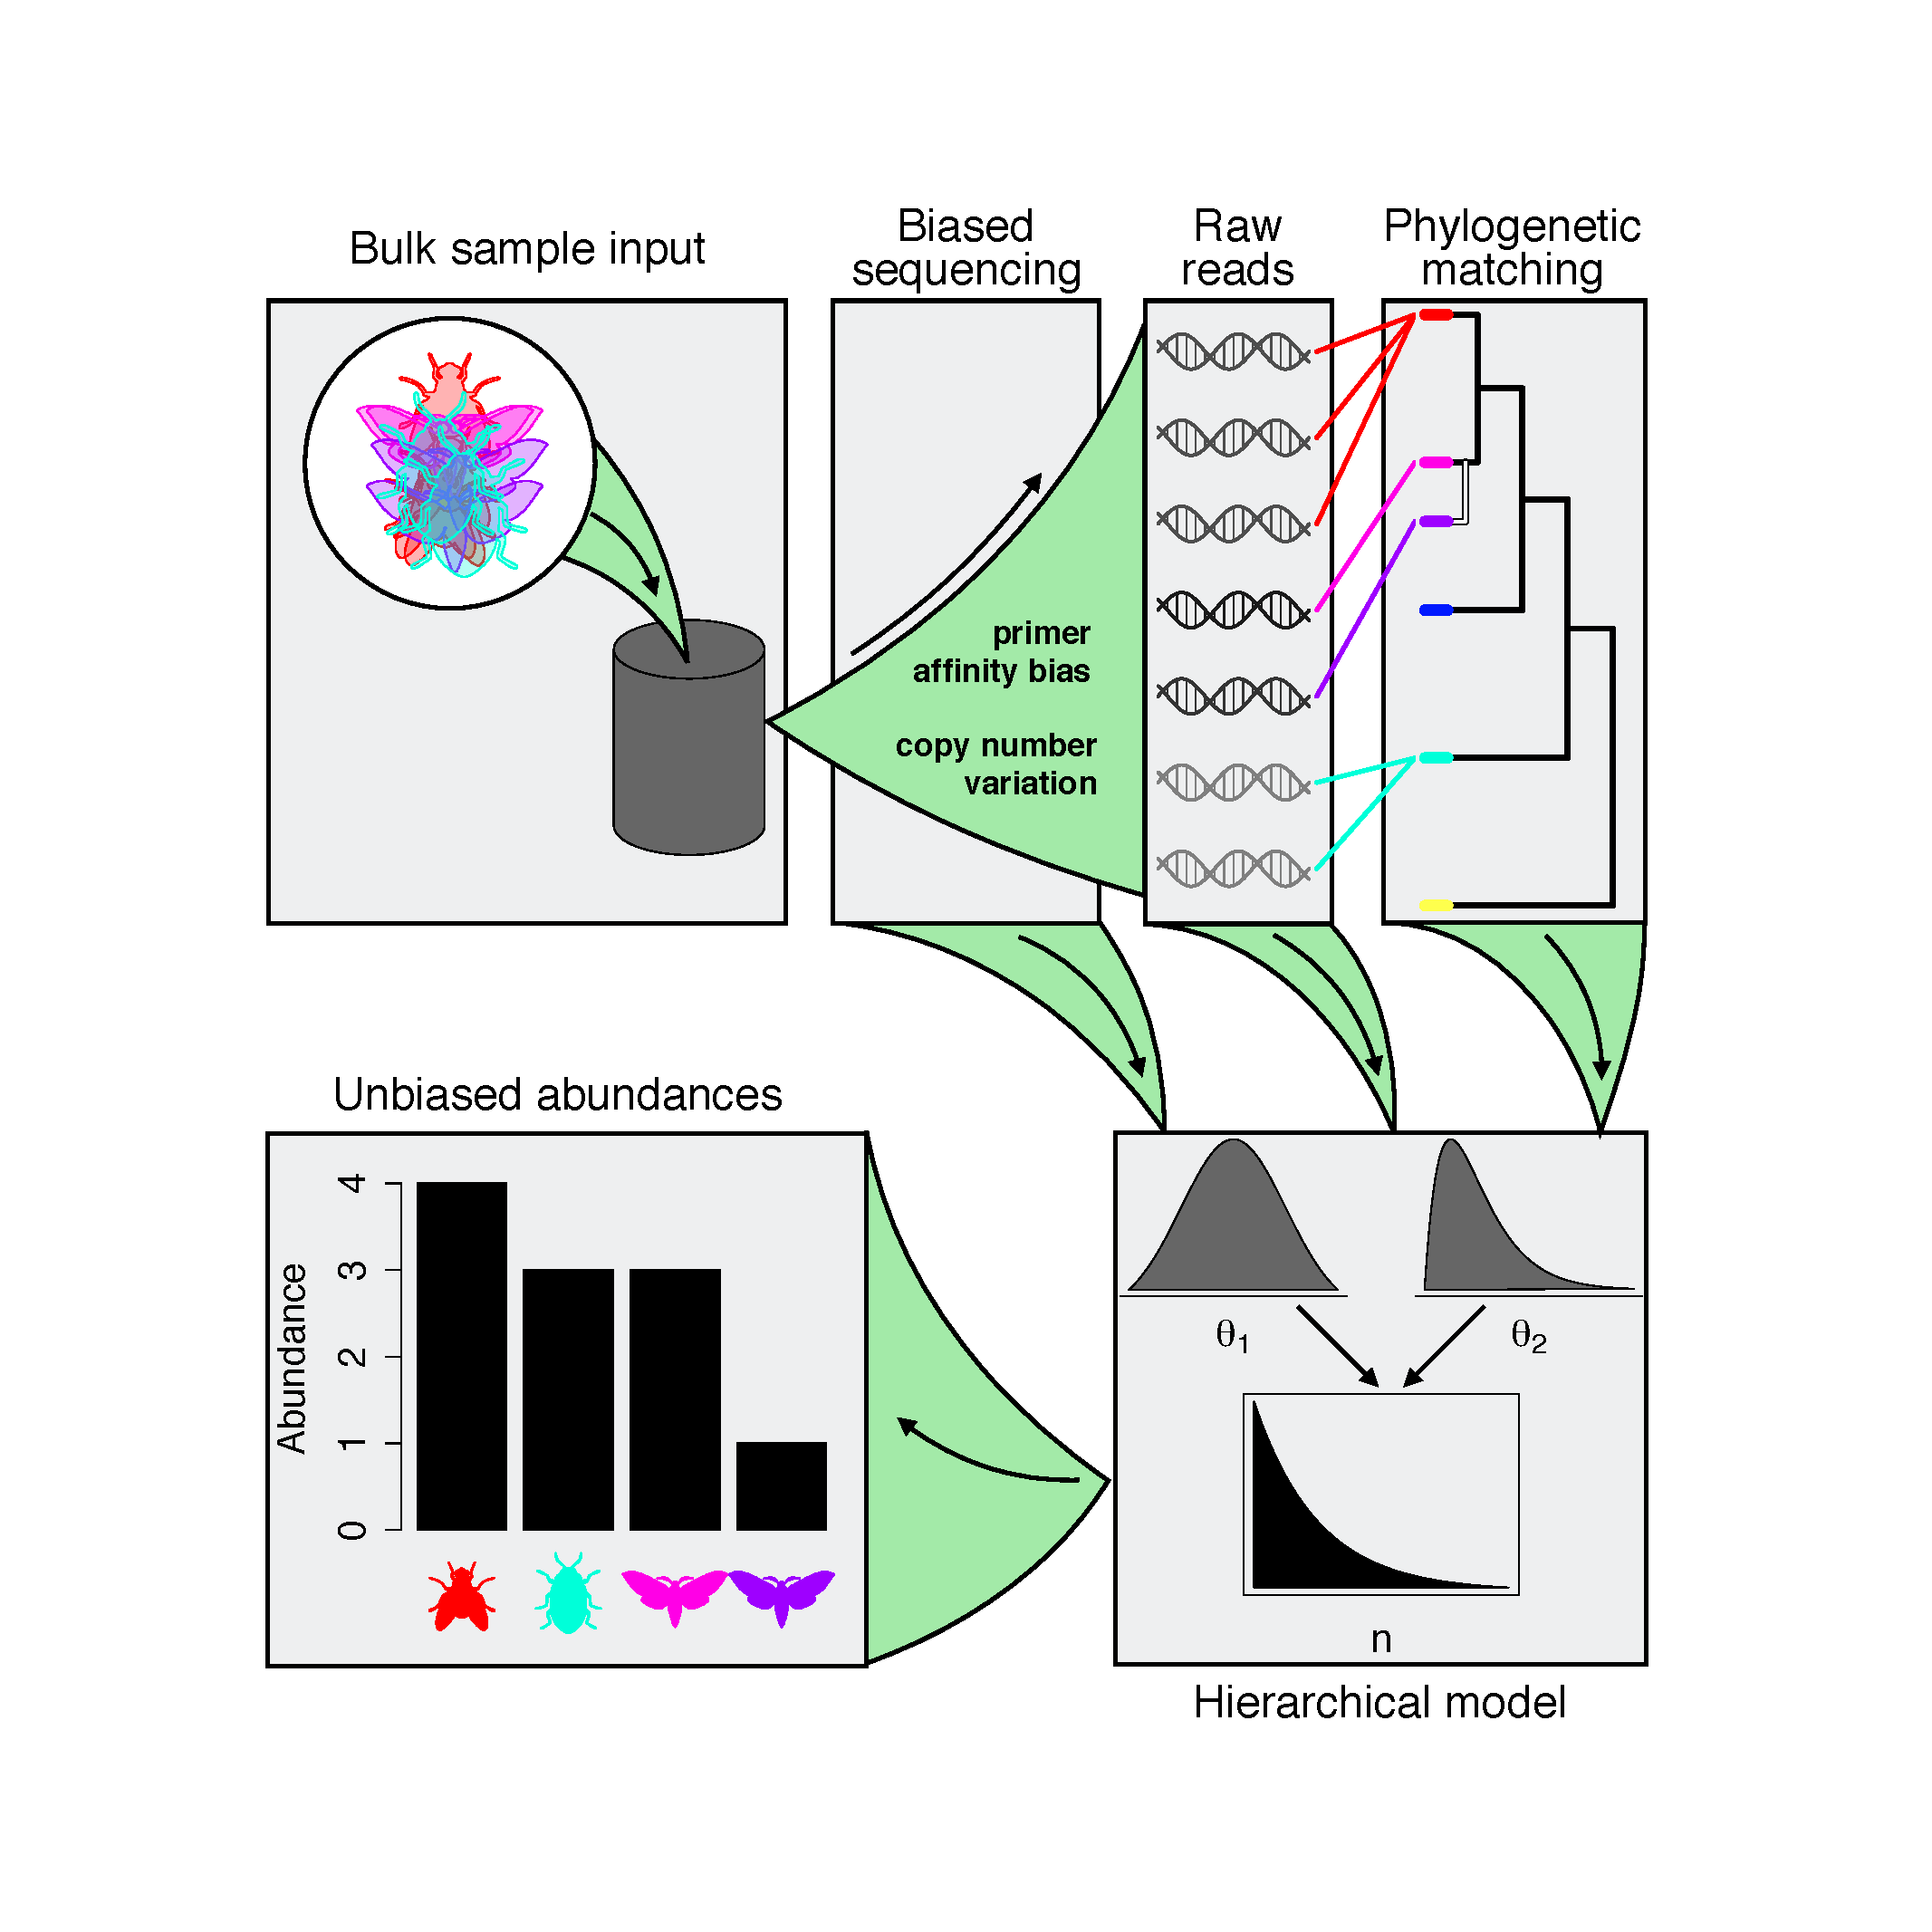
\includegraphics[scale=0.3]{../figs/fig_metab.pdf}
  \end{center}
  \caption{Pipeline for generating and analyzing metabarcoding
    samples.}
  \vspace{0pt}
\end{wrapfigure}
%

Next generation sequencing technology has ushered in a revolution in
evolutionary biology and ecology. The large scale recovery of species
richness, food web structure, cryptic species, identification of
juveniles and hidden diversity, e.g. internal parasitoids, promise
unprecedented new insights into ecosystem function and assembly
\citep{krehenwinkel2016, shokralla2015, gibson2014,
  taberlet2012}. While species richness can be routinely identified by
sequencing bulk samples, estimating species abundance remains
challenging \citep{elbrecht2015} and severely limits the application
of metabarcoding to many studies. We are developing wet lab and
bioinformatic methods to overcome this issue and revolutionize the
generation of ecological and genetic data ({\bf RO4}). We will apply this
approach primarily to bulk arthropod collections, while complementary
approaches will be used to reconstruct microbial diversity, and
networks between plants, arthropods and microbes. Our novel pipeline
consists of three steps (Fig. \ref{fig:metab}):
\begin{enumerate}
\item Extraction and sequencing of pooled community samples
\item Matching the resulting sequences to a reference phylogeny for
  identification
\item Using Bayesian hierarchical models to reconstruct unbiased
  estimates of abundance
\end{enumerate}

Step (1) is already well developed \citep{krehenwinkel2016,
  shokralla2015, gibson2014, taberlet2012}; steps (2-3) will be
developed into an open source {\tt R} package that allows users to
implement these methods in their study systems.  We propose that our
open source pipeline can be implemented across NEON sites to generate
both taxonomic and phylogenetic data for focal taxa.

Preliminary results from controlled experiments show there is a strong
correlation between amount of arthropod tissue sequenced and total
number of reads; however, this relationship is variable across taxa. A
Bayesian model is able to capture this variability across taxa and
thus indicates the success of more general applications of the
modeling approach to field collections.

\paragraph{(1) Extraction and sequencing of pooled community samples.}
We will generate sequence information for mixed arthropod community
samples, collected across precipitation gradients on the Hawaiian
Archipelago. The samples will be roughly pre-sorted taxonomically and
grouped into different body size classes to minimize the confounding
factors of abundance and body size in determining amount of DNA per
taxon. We will use amplicon sequencing of the COI barcoding region
\citep{taberlet2012} which has shown the greatest reliability in
preliminary trials.


\paragraph{(2) Matching the resulting sequences to a reference
  phylogeny for identification.}
In order to resolve the taxonomy of sequences derived from mixed
samples we are developing a library of the barcoding region for
species across the Hawaiian archipelago, such that unknown sequences
can be phylogenetically matched to the reference library.
Sequences not found in the tree of all reference sequences will be
grafted and their status as a unique operational taxonomic unit
assessed using a cutoff of 3\% divergence (Fig. \ref{fig:metab}).
These bioinformatic steps will be included in the {\tt R} package.

In collaboration with taxonomist and ecologist on Hawaii, we are
currently working on generating the barcode reference library for a
diverse range of several hundred Hawaiian arthropod taxa. These taxa
were sampled across the chronosequence of the Hawaiian Archipelago
(Fig. \ref{fig:map}). DNA is extracted from each taxon and reference
sequence generated for the mitochondrial COI barcoding region. To
achieve a comprehensive sampling of the Hawaiian arthropod diversity,
samples from environmental gradients (e.g. precipitation) will be
included in this reference collection. Such gradients have been shown
to have a profound influence on community composition on Hawaii
\citep{zimmerman2012}.

In order to build a robust phylogenetic backbone for our reference
library, the genomic DNA extracts for all species will be sequenced
using the Illumina HiSeq2500. An assembly of the resulting reads
promises to generate near complete mitochondrial genomes and nuclear
ribosomal clusters of each taxon. To support the Illumina short read
assemblies, we will generate long read information by PacBio
sequencing. The resulting sequence information will allow us to
reconstruct a well resolved community-phylogenetic framework for
ecological hypothesis testing.  These same specimens will also be used
to quantify the microbiomes and feeding habits of hundreds of
arthropod species across our sites (discussed further in section
``Quantifying networks of microbes, arthropods and plants'').

\paragraph{(3) Using Bayesian hierarchical models to reconstruct
  unbiased estimates of abundance}
Bayesian hierarchical models permit inference of key quantities
(e.g. abundance) while accounting for multiple sources of error and
leveraging heterogeneous data types to facilitate inference
\citep{royleDorazio}.  The goal of hierarchically modeling
metabarcoding data is to estimate the abundances of species while
correcting for known biases inherent in amplicon-based sequencing.  We
will account for bias from copy number variation and primer affinity
\citep{elbrecht2015} by directly modeling it, while also using data on
the total number of individuals being sequenced, their body sizes, and
the phylogenetic relationship between their sequences to constrain the
estimates to be more accurate.  Furthermore, information from
controlled experiments (for example making mock communities of known
composition and sequencing those) can be used to constrain prior
distributions and obtain even more accurate abundance estimates.


\subsection{Quantifying networks of microbes, arthropods and plants}

Using the specimens reserved from metabarcoding (i.e. those used to
build the reference library and phylogenetic backbone) we will
sequence the microbial associates of each species and their gut
contents, for herbivorous arthropods.  These sequences will allow us
to reconstruct the networks between arthropods and their microbial
associates as well as herbivorous arthropods and their plant hosts.
We will additionally reconstruct microbial networks based on
covariance between prevalence of microbial taxa in samples using
established approaches \citep{kurtz2015}.


\section{Broader Impacts}
The research will train 3 postdocs, including one who will serve as PI
for the proposal and gain experience in leading the effort. It will
also train 2 graduate students, and 12 or more undergraduates, at the
intersection between macroecology and evolution, and across microbes
to macroorganisms.

We will use the rich natural and dynamic landscape of Hawaii, and the
acute environmental issues affecting the environment, to build a
program of education and outreach. The PIs are already well positioned
for such activities. The primary areas we plan to develop are:
\begin{enumerate}
\item Experiences for undergraduates and Masters students. We will build
  research experiences for undergraduates and Masters students from
  both the University of Hawaii Hilo (minority-serving, 24\% Hawaiian)
  and the University of Hawaii Maui College (also minority-serving,
  37\% Hawaiian). At the University of Hawaii Hilo, we will connect
  with the Ecology, Evolution and Conservation Biology (EECB) and
  Tropical Conservation Biology and Environmental Science program
  (TCBES, \url{tcbes.uhh.hawaii.edu}); Gillespie is already an
  Affiliate Faculty member of TCBES. The EECB and TCBES Programs give
  high priority to the recruitment and training of students from
  groups under-represented in sciences with an emphasis on Native
  Hawaiian and Pacific Islanders. These efforts will be facilitated
  through the Pacific Internship Programs for Exploring Science
  (PIPES) program (\url{www.uhh.hawaii.edu/uhintern}), a UH
  Hilo program designed to connect underrepresented undergraduate
  students, especially Native Pacific Islanders, to research
  internship opportunities relating to environmental issues in Hawaii;
  we will recruit undergraduates through this program (see letter
  attached). The research will involve each of the undergraduates
  coming out into the field with researchers involved in the
  project. We have already established close ties with Cathy
  Davenport, a faculty member at the University of Hawaii Maui College
  (see letter attached). The students will assist in field sampling at
  specific locations associated with the main sampling locations for
  the overall grant program. Specific projects that the students could
  conduct are as follows (i) comparison of species diversity of key
  groups of arthropods on young versus old lava flows; (ii)
  relationship between substrate age and diversity of targeted
  arthropod species; and (iii) analysis of the effects of forest
  fragmentation (natural and human) on species diversity of targeted
  arthropod species.
\item Experiences for High school and Middle School students. The USDA
  Forest Service co-leads, with the University of Hawaii at Manoa, a
  ``Teaching Change Program.'' This program features over-night
  immersive learning experiences to students by bringing students to
  natural areas of Hawaii Island. The current two-day curriculum
  focuses on linking phenology, conservation biology, and climate
  change on the island of Hawaii. Each month students visit a site to:
  (i) learn about native forest ecosystem ecology, including
  disturbance regimes and the general concept of change; (ii) learn
  about human-induced climate change and its potential impact on
  native ecosystems; (iii) measure plant phenology and publish these
  data with the USA National Phenology Network; and (iv) participate
  in native forest bird research. With monthly trips, this program is
  generating a unique tropical montane forest dataset on plant
  phenology and exposes students to: (i) native ecosystems that they
  would never otherwise have the opportunity to visit; (ii) the
  concept of plant and avian phenology and its utility for monitoring
  native ecosystems; and (iii) the concept of change, including
  anthropogenic climate change. Over the past four years the program
  has served 400+ students. The program has a particular focus on
  underprivileged and underrepresented youth from Hawai'i. It also
  provides Teacher Training Workshops for local teachers and offers
  annual Conservation Career Days for students and their families to
  learn about professional and educational opportunities in Hawai'i in
  conservation biology and natural resource management to inspire and
  empower the next generation of land managers in Hawai'i.
\item Land Management Professionals. Fieldwork in Hawaii will be timed
  to coincide with the annual Hawaii Conservation Conference, the
  largest gathering of people ($\gg 1000$ participants) actively involved
  in the protection and management of Hawaii's environment (see
  \url{hawaiiconservation.org}). The goal of the conference is to
  foster interaction between natural resource managers and the
  scientific community. In addition to holding a workshop to present
  and discuss our results at the conference, we plan to have one
  afternoon of round table discussion for the local community on the
  island of Hawaii, allowing a smaller group from university, state
  (DLNR), private (The Nature Conservancy of Hawaii), and federal
  (USGS, USFS, USDA, USFWS) agencies, and others, to discuss the work,
  its results and significance.
\end{enumerate}

Besides working with local communities in Hawaii, we also plan to make
use of avenues for outreach and education at UC Berkeley. We plan to
develop a diverse, high-performing, and interdisciplinary
\citep{cheruvelil2014, goring2014} community of researchers as we have
done in the past, that includes postdocs, graduate, and undergraduate
students. In addition, we plan to:
\begin{enumerate}
\item Work with staff at the UC Berkeley Natural History Museums in
  the development of material for the Understanding Evolution
  (evolution.berkeley.edu) web site, designed for science
  teachers of all grade- and experience-levels. The system, which
  couples elements of evolution and ecology, field and laboratory,
  theoretical and empirical, provides an opportunity to convey some
  essential yet complex concepts in a relatively straightforward
  manner.
\item Use the forum provided by LBNL's Open House for connecting to
  the local community (\url{www2.lbl.gov/openhouse}) and
  especially the Science at the Theater
  (\url{uctv.tv/scienceatthetheater}) events.
\end{enumerate}

\section{Results from prior funding}

\paragraph{Chase:} DEB 0949984 Mechanisms of species-area
relationships in Ozark glades. 2010-2015, \$748,046.00 (co-PI; Tiffany
Knight, PI). Intellectual merit. The observation that larger areas
typically support more species is the basis for the species-area
relationship, one of the oldest and best known relationships in
ecology. Nevertheless, the mechanisms underlying this relationship
remain poorly understood. Specifically, the lower diversity found in
small habitats is often a consequence of there being fewer rare
species in those habitats than would be expected based on
sampling. This grant funded a long-term, large-scale experiment in
experimentally restored Ozark Glade communities. Population and
community-level patterns were monitored, providing important
implications for understanding, and trying to mitigate, biodiversity
loss from small habitats, especially loss of rare species. {\bf
  Broader Impacts:} The primary impact of this research outside of
basic understanding of restoration ecology principles was to engage
cohorts of undergraduate and high school students (many from
underrepresented groups) in genuine research experiences at the field
station. More than 50 such students participated in research in these
glades over the course of the experiment, as well as 5 PhD students
and 3 postdoctoral fellows. Papers to date: \citep{burkle2012,
  chase2013, powell2013, schuler2015}, with 6 others currently
submitted or in revision.

 
\paragraph{Gillespie:} DEB 1241253 Dimensions: A community level
approach to understanding speciation in Hawaiian lineages. 2013-2018
(PI; co-PIs John Harte, Rasmus Nielsen, Patrick O’Grady), \$1,181,407
to UC Berkeley (collaborators in Cornell, University of Hawaii Hilo, U
Maryland, Pacific Ecoinformatics, for a total award of
\$1,999,910). Intellectual Merit. This project aims to transform
understanding of the impact of the dynamic community on biodiversity
by integrating (1) evolutionary models, and (2) macro-ecological
theory. The synergy between the two approaches is made possible
through the use of a habitat chronosequence, and corresponding
space-for-time substitution, provided by the dynamic geomorphology of
the young islands of the Hawaiian archipelago. We selected 6 plots in
each of $15+$ sites and are sorting thousands of arthropod specimens
while creating an mtDNA barcode library and testing metabarcoding
approaches. From these data we are estimating macroecological metrics
and conducting food web analysis. For focal lineages, genomic data is
providing information on population differentiation over the island
chronology for different trophic groups. {\bf Broader Impacts:} New
species are being discovered and research is integrated into
education; trained 7 postdocs, 10 graduate students, 14
undergraduates, and one high school student in the last year and gave
$> 11$ presentations at scientific meetings. To date this work has
produced 10 papers \citep{rominger2016, rominger2015,
  krehenwinkel2016, gillespie2014, shaw2016, gillespie2016,
  brewer2015, brewer2014, warren2015, gillespie2013}.

\paragraph{Gruner:} DEB-1020007 Collaborative Research: Interactive
effects of predation and ecosystem size on arthropod food webs in
Hawaiian forests fragmented by lava flows. 2010-2015 (collaborative
PIs Tad Fukami, David Flaspohler, Christian Giardina), \$329,949 to U
Maryland (collaborators at Stanford, Michigan Tech, and US Forest
Service, for a total award of \$1,213,843). Intellectual Merit. This
project examined forest food webs in naturally fragmented landscapes
on Hawaii Island over a 100-fold ecosystem size gradient. Our
overarching objective was to test the contingent effects of an
invasive omnivore, the black rat Rattus rattus, on bird population
dynamics, arthropod food webs, and ecosystem processes. By eliminating
rats from fragments up to 12 ha in size in a 4-yr press experiment,
and independently excluding birds from tree canopies, we provided
evidence for non-consumptive effects of rats in altering bird foraging
behavior and their impacts on arthropods. This work has produced 10
peer-reviewed papers \citep{massol2011, vaughn2013, knowlton2014,
  vaughn2014, vaughn2015, knowlton2016, vannette2016}, with three more
in review or in revision. {\bf Broader Impacts:} More than 25
undergraduate students participated as interns and paid assistants in
this research. Two students were mentored through the Pacific
Internship Programs for Exploring Science (PIPES) program, which is
committed to recruiting and retaining local Hawaiian students in
research. Three students completed MS degrees at University of Hawaii
Hilo (Phifer, 2012; Mueller et al. In review; Wilson Rankin et al. In
review), one PhD project is ongoing at Stanford University, and three
postdocs were mentored and placed in subsequent positions. The project
was featured in volume 16 (2012) of the {\it Natural Inquirer}, a
middle school science education journal produced by the US Forest
Service.



%% suppresses bibliography, then make tex file to compile .bbl in separate doc
\bibliographystyle{unsrtnat}
\setbox0\vbox{\bibliography{../macrosystems.bib}}


\end{document}



